%\documentclass[12pt]{aastex}
\documentclass[iop]{emulateapj}
%\documentclass{article}
\usepackage{draftwatermark}
\usepackage{paralist}
\shorttitle{MRI in massive disks}
\shortauthors{M-K. Lin}

\usepackage{amsmath}
%\usepackage{url}
\usepackage{bm}
%\usepackage[font=small,format=plain,labelfont=bf,up,textfont=it,up]{caption}
\newcommand{\p}{\partial}
\newcommand{\lmax}{l_\mathrm{max}}
\newcommand{\sbar}{\bar{\sigma}} 
\newcommand{\imgi}{\mathrm{i}} 
\newcommand{\ii}{\mathrm{i}}
\newcommand{\C}{\mathcal{C}^\lambda}
\newcommand{\wop}[1]{\mathcal{V}^{(#1)}}
\newcommand{\avg}[1]{\langle{#1}\rangle}
\newcommand{\zhat}{\hat{z}}
\newcommand{\rhat}{\hat{r}}
\newcommand{\he}{\mathcal{H}}
\newcommand{\amp}{\mathcal{A}}
\newcommand{\dd}{\delta}
\newcommand{\real}{\operatorname{Re}}
\newcommand{\imag}{\operatorname{Im}}
\newcommand{\sgn}{\operatorname{sgn}}
\newcommand{\zmax}{Z_s}
\newcommand{\wbar}{\tilde{W}}
\newcommand{\qbar}{\tilde{Q}}
\newcommand{\dbigH}{\frac{H^\prime}{H}}
\newcommand{\Rp}{\frac{\rho_0^\prime}{\rho_0}}
\newcommand{\Fp}{\frac{g^\prime}{g}}
\newcommand{\Rpp}{\frac{\rho_0^{\prime\prime}}{\rho_0}}
\newcommand{\Fpp}{\frac{g^{\prime\prime}}{g}}
\newcommand{\ils}{L_s^{-1}}
\newcommand{\ilp}{L_p^{-1}}
\newcommand{\ihp}{H_p^{-1}}
\newcommand{\ihs}{H_s^{-1}}
\newcommand{\ciso}{c_\mathrm{iso}}
\newcommand{\csmid}{c_{s0}} 
\newcommand{\hiso}{h_\mathrm{iso}}
\newcommand{\Hiso}{H_\mathrm{iso}}
\newcommand{\zeus}{\texttt{ZEUS-MP }}
\newcommand{\rsph}{r_\mathrm{sph}}
\newcommand{\dvx}{\dd v_x}
\newcommand{\dvy}{\dd v_y}
\newcommand{\dvz}{\dd v_z}
\newcommand{\dbx}{\dd B_x}
\newcommand{\dby}{\dd B_y}
\newcommand{\dbz}{\dd B_z}
\newcommand{\w}{ \tilde{W}}
\newcommand{\dphi}{\dd \Phi}
\defcitealias{lin12}{L12} 

\begin{document}

 \title{Resistive magneto-rotational instability in massive
  protoplanetary disks}


\author{Min-Kai Lin}
\affil{Canadian Institute for Theoretical Astrophysics,
  60 St. George Street, Toronto, ON, M5S 3H8, Canada}
\email{mklin924@cita.utoronto.ca}

\begin{abstract}

\end{abstract}

\section{Introduction}


\section{Local disk model}\label{setup}
We study the local stability of an inviscid, self-gravitating and
magnetized fluid disk orbiting a central star with
potential $\Phi_*(r,z)$, where $(r,\varphi,z)$ are cylindrical
co-ordinates from the star. We use the shearing box approximation     
\citep{goldreich65b} to consider a small patch of the disk at
a fiducial radius $r=r_0$. The local frame rotates at angular velocity 
$\Omega_0=\Omega(r_0,0)$ about the star, where $r\Omega^2 =
\p\Phi_*/\p r$. We also define $S\equiv-r\p\Omega/\p r$ as the local shear
rate and $\Omega_z^2\equiv\p^2\Phi_*/\p z^2$ as the square of the
local vertical frequency. 

A Cartesian co-ordinate system $(x,y,z)$ is set
up in this local frame, corresponding to the radial, azimuthal and vertical
directions of the global disk, respectively. The shearing box fluid
equations read 
\begin{align} 
  &\frac{\p\rho}{\p t}+\nabla\cdot(\rho\bm{v}) = 0,\\
  &\frac{\p \bm{v}}{\p t} + \bm{v}\cdot\nabla\bm{v} +
  2\Omega_0\hat{\bm{z}}\times\bm{v} = - \frac{1}{\rho}\nabla\Pi +
  \frac{1}{\rho\mu_0}\bm{B}\cdot\nabla\bm{B}
  -\nabla\Phi,\\
  &\frac{\p\bm{B}}{\p t}= \nabla\times\left(\bm{v}\times\bm{B} -
  \eta\nabla\times\bm{B}\right), 
\end{align}
where $\rho$ is the density field; $\bm{v}$ is the total velocity in
the local frame; $\bm{B}$ is the magnetic field which satisfies
$\nabla\cdot~\bm{B}=0$; $\Pi \equiv P +
|\bm{B}|^2/2\mu_0$ is the total pressure, and $\mu_0$ is the vacuum
permeability. We choose a barotropic equation of state, specified
below, so that the gas pressure is given by $P=P(\rho)$. The
resistivity $\eta$ is either uniform or a prescribed function of
height. 


The total potential is $\Phi = \Phi_\mathrm{ext} + \Phi_d$, where
\begin{align}
  \Phi_\mathrm{ext}(x,z) = -\Omega_0 S_0 x^2 +
  \frac{1}{2}\Omega_{z0}^2z^2 
\end{align}
is the effective external potential (central plus centrifugal) in the
shearing box approximation, where $S_0\equiv ~S(r_0,0)$ and
$\Omega_{z0}\equiv\Omega_z(r_0,0)$; 
and the gas potential $\Phi_d$ satisfies Poisson's equation
\begin{align}
  \nabla^2\Phi_d = 4\pi G \rho, 
\end{align}
where $G$ is the gravitational constant. For clarity, hereafter we
drop the subscript $0$ on the frequencies. 



\subsection{Equilibrium disk} 
The unperturbed disk is steady and described by
$\rho=~\rho(z)$, $\bm{B} = B_z\hat{\bm{z}} + B_y\hat{\bm{y}}$ where
$B_{y,z}$ are constants and the toroidal field strength is
$B_y=\epsilon B_z$. The equilibrium 
velocity field is $\bm{v} = -Sx\hat{\bm{y}}$. We consider Keplerian
disks so that $S = 3\Omega/2$ and the epicycle frequency 
$\kappa\equiv\sqrt{2\Omega(2\Omega-S)}=\Omega=\Omega_z$.  
We assume a thin disk and neglect the radial component of the
self-gravitational force in the unperturbed disk.    

The equilibrium density field is obtained by solving
\begin{align}
  &0=\frac{1}{\rho}\frac{d P}{dz} + \Omega_z^2z + \frac{d\Phi_d}{dz},\label{eqm_eqns1}\\
  &\frac{d^2\Phi_d}{dz^2} = 4\pi G \rho.\label{eqm_eqns2}
\end{align}
We consider \begin{inparaenum}[(i)]
\item isothermal disks with $P=c_{s0}^2\rho$\label{iso_eos}; 
\item polytropic disks with $P=K\rho^2$ with $K=c_{s0}^2/2\rho_0$;
\end{inparaenum}
where $\rho_0\equiv\rho(0)$ is the midplane density.
The sound speed $c_s\equiv\sqrt{dP/d\rho}$ 
so that $c_{s0}$ is the global sound speed in the isothermal disk, and
is the midplane sound speed in the polytropic disk. For the polytropic
disk the disk thickness $H$ is such that $\rho(H)=0$. Since the
isothermal disk has no surface, we define $H$ such that
$\rho(H)=10^{-2}\rho_0$. A non-dimensional
measure of the disk thickness is given by 
\begin{align}
  f^{-1} = \frac{H\Omega}{\csmid}, 
\end{align}
and $f$ will appear in subsequent discussions. 


We solve for $\hat{\rho}\equiv\rho/\rho_0$ with 
boundary conditions $\hat{\rho}=1$ and $d\hat{\rho}/dz=0$  at $z=0$. This
is done numerically for isothermal disks and analytically for the
polytropic disk (see Appendix \ref{appen1}). Examples of density
profiles are shown in Fig. \ref{eqm_den}. The normalized density field
is weakly dependent on the strength of self-gravity provided the
$z$-axis is appropriately scaled. 


\begin{figure}
  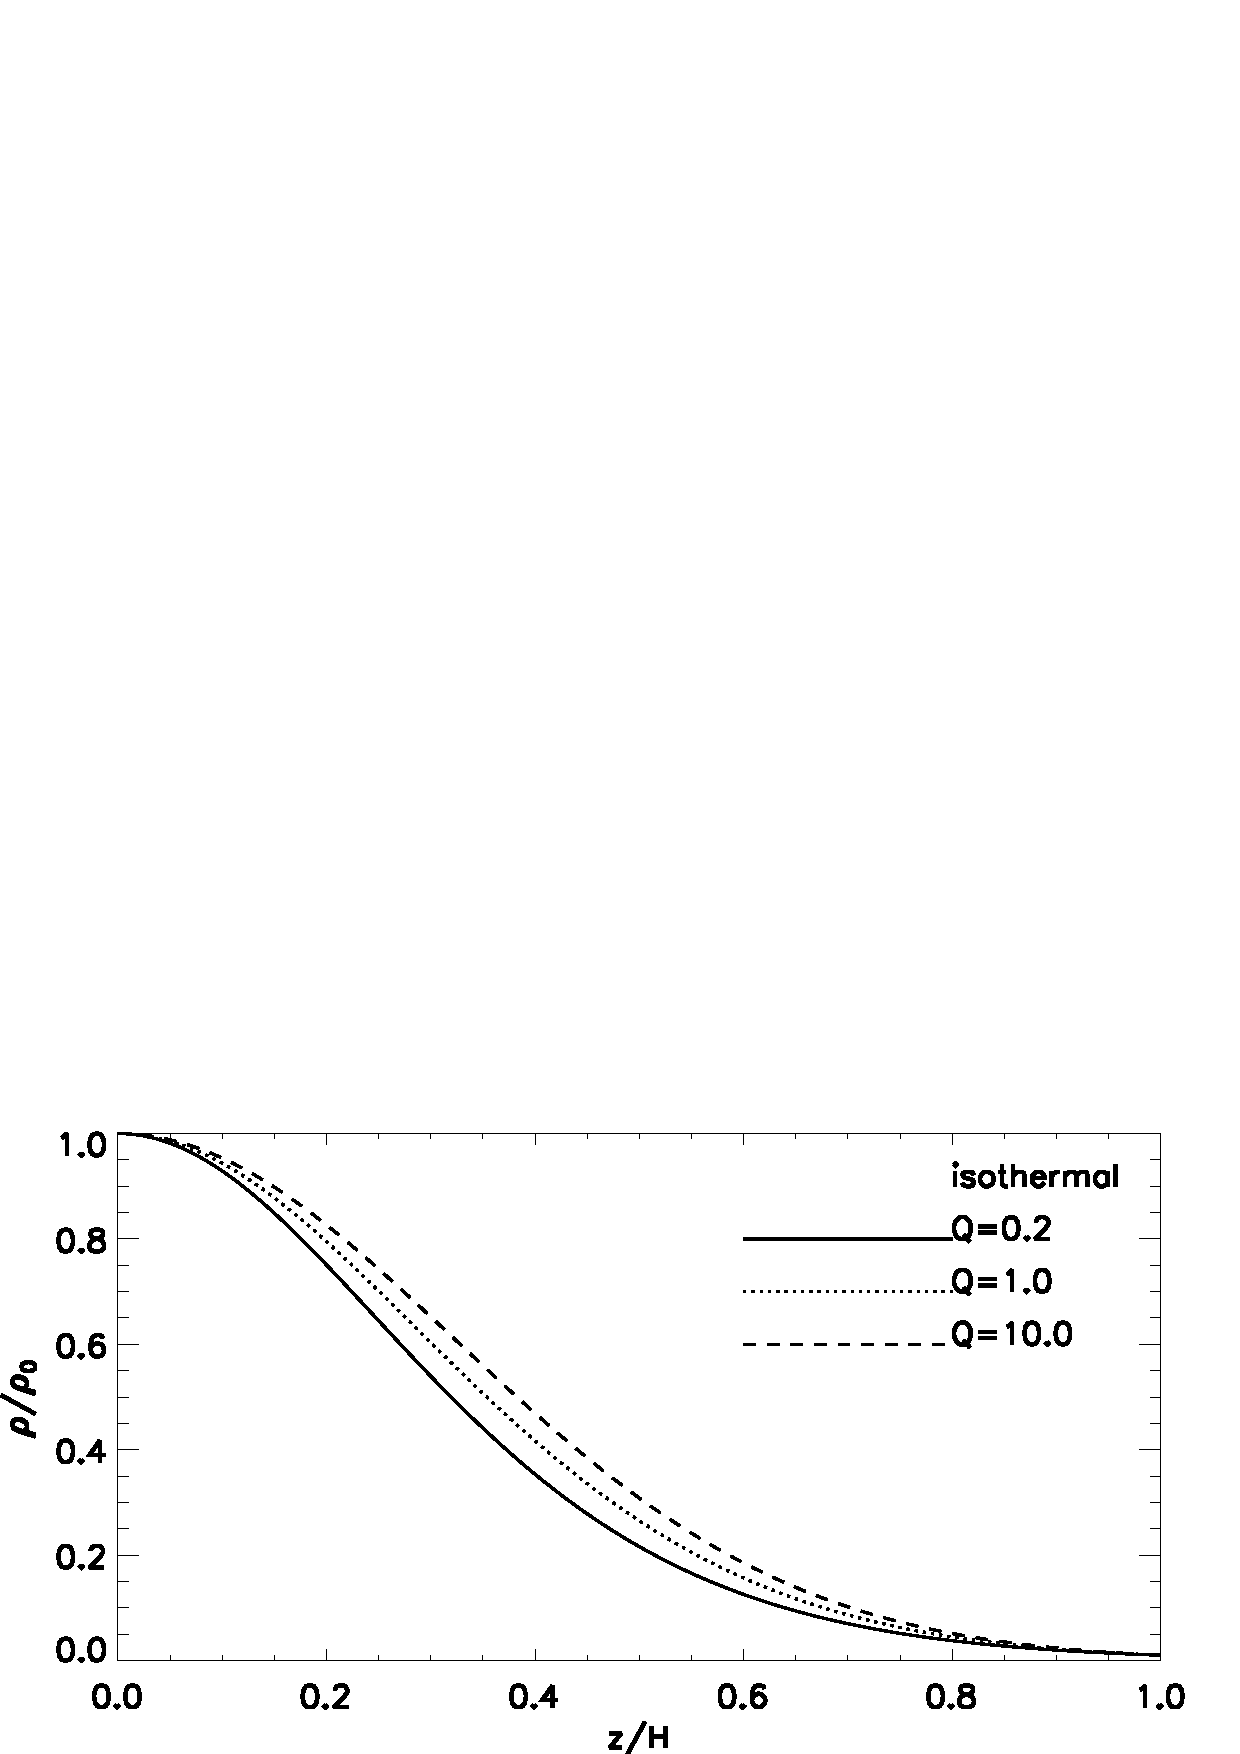
\includegraphics[width=\linewidth,clip=true,trim=0cm 1.5cm 0cm
    0cm]{figures/compare_iso_density} 
  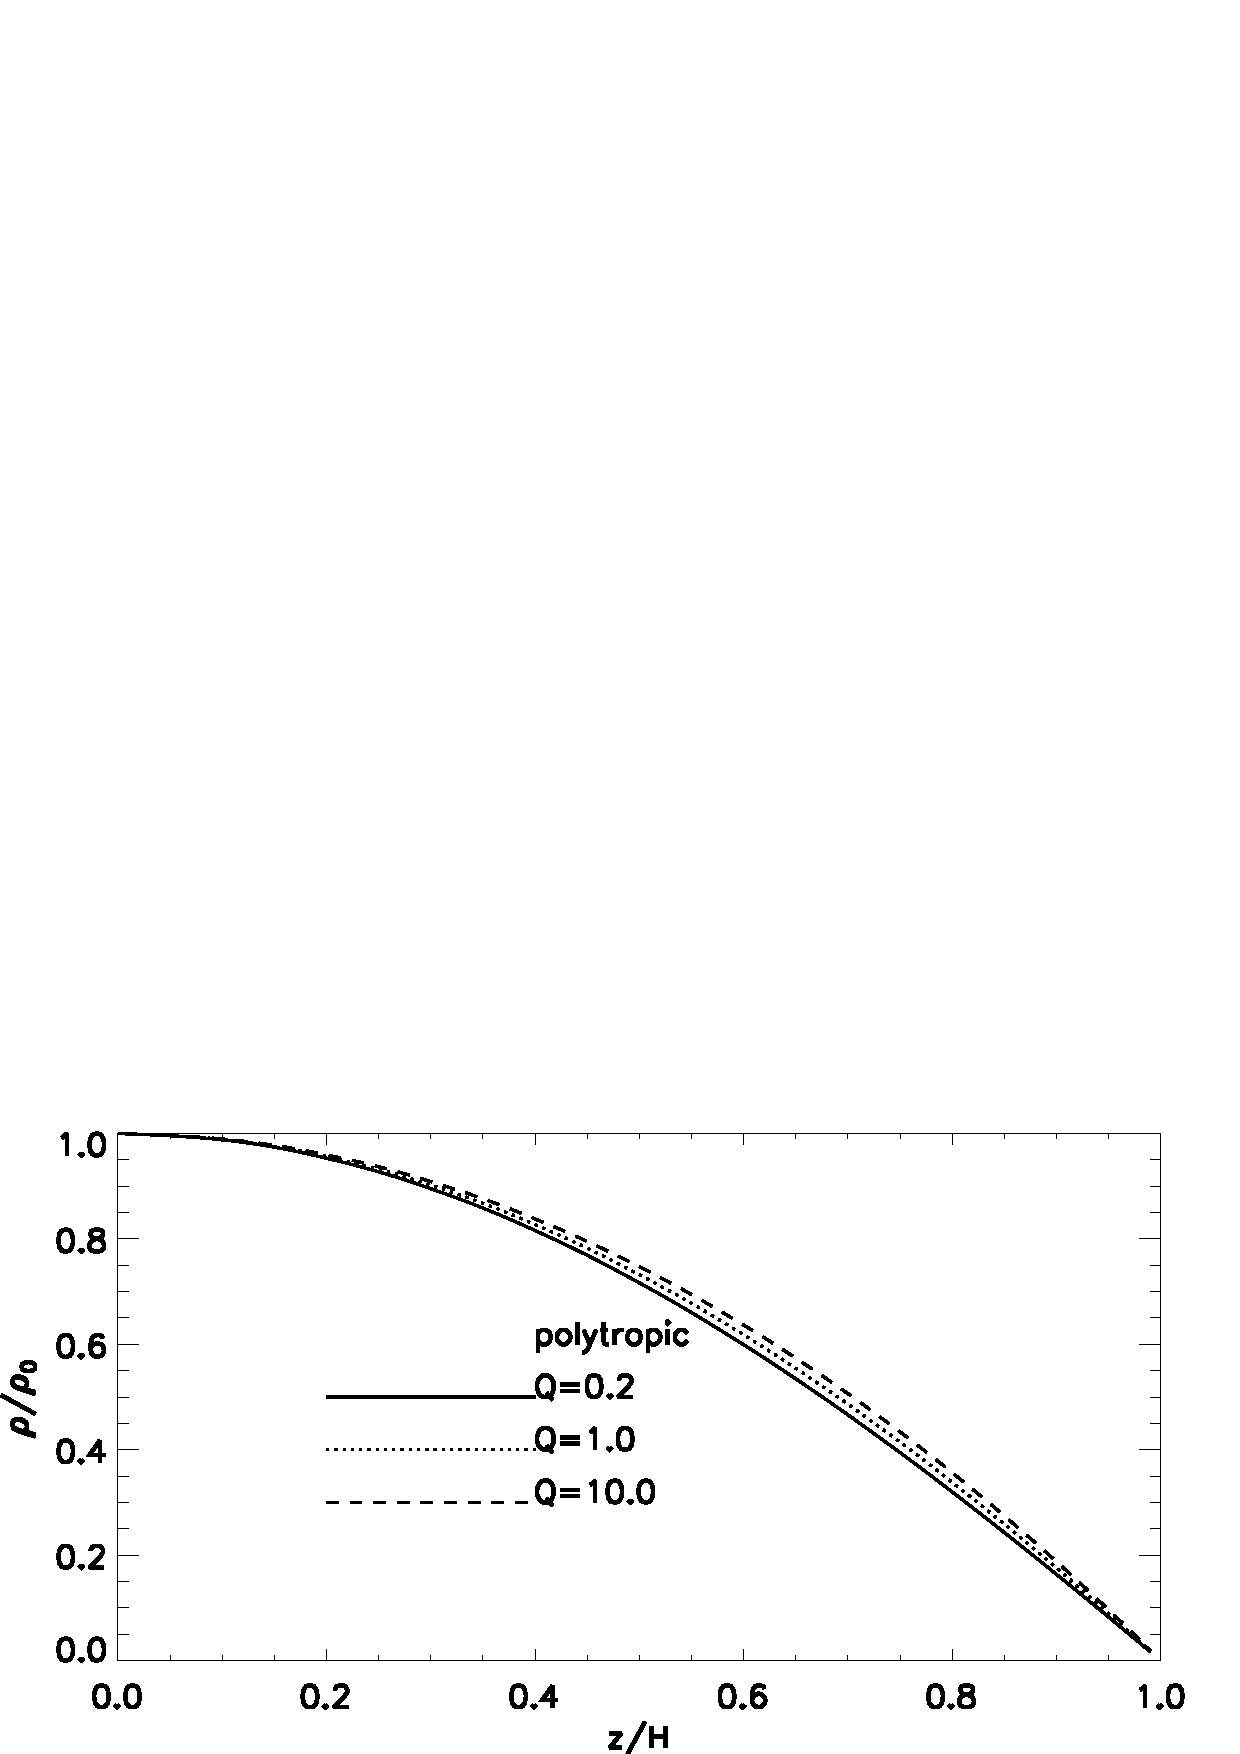
\includegraphics[width=\linewidth,clip=true,trim=0cm 0cm 0cm
    0.9cm]{figures/compare_poly_density} 
  \caption{Equilibrium density field from solving Eq. \ref{eqm_eqns1}
    --- \ref{eqm_eqns2} subject to an isothermal (top) and polytropic
    (bottom) equation of state. Note that the normalization for the
    horizontal axis also depends on the strength of self-gravity,
    i.e. $H=H(Q)$ and is an increasing function of $Q$. 
    \label{eqm_den}}
\end{figure}


\subsection{Resistivity profile}\label{resis_profile}
We adopt constant resistivity or a 
resistivity prescription such that $\eta(z)$ increase {\bf towards} the
midplane. In the latter case, we follow \cite{fleming03} and use 
the resistivity profile 
\begin{align}
  \eta(z) =
  \sqrt{2}\eta_0\left[\exp{\left(-g_+\right)}+\exp{\left(-g_-\right)}\right]^{-1/2},  
\end{align}
where
\begin{align}
  &g_\pm(z) =  \frac{\Sigma_\pm(z)-\Sigma_0}{\Sigma_*}, \\
  &\Sigma_\pm(z) = \int_{\pm z}^\infty\rho(z^\prime)dz^\prime, \label{sigma_pm}
\end{align}
and $\Sigma_0\equiv\Sigma_{\pm}(0)$, so that $g_\pm(0)=0$ and $\eta_0 
= \eta(0)$. The constant $\Sigma_*$ is chosen such that 
\begin{align}
  \cosh{\left(\frac{\Sigma_0}{\Sigma_*}\right)} =
  \left[\frac{\eta_0}{\eta(\infty)}\right]^2,
\end{align}
and we define $\eta_0/\eta(\infty)\equiv A$ as the conductivity 
boost factor from the midplane to the disk surface. We remark that
once $\rho$ and $d\rho/dz$ are obtained from
Eq. \ref{eqm_eqns1} --- \ref{eqm_eqns2}, the integration for
Eq. \ref{sigma_pm} can be performed implicitly by using Poisson's 
equation. 

We use the Elsasser number $\Lambda$ a non-dimensional measure of
conductivity,
\begin{align} 
  \Lambda \equiv \frac{v_A^2}{\eta\Omega},
\end{align}
where $v_A \equiv B_z/\sqrt{\mu_0\rho}$ is the vertical Alfven speed. 
Because of the density stratification, the Elsasser number 
increases with height even for constant resistivity. The disk may be
considered ideal where $\Lambda \gtrsim 1$. 


\subsection{Disk parameters}
%The main parameters describing the resistive, self-gravitating
%shearing box is as follows. 
The strength of self-gravity is
parametrized by 
\begin{align}
  Q \equiv \frac{\Omega^2}{4\pi G\rho_0}
\end{align}
\citep{mamat10}, which is used to set the midplane density $\rho_0$. 
A relation between $Q$ and the Toomre parameter for gravitational
instability of razor-thin disks, $Q_\mathrm{2D}$, is described in
Appendix \ref{q3d2d}.  

The plasma $\beta$ measures the inverse strength of the  
magnetic field 
\begin{align}
  \beta \equiv \frac{\csmid^2}{v_{A0}^2} =
  \frac{\csmid^2\mu_0\rho_0}{B_z^2},  
\end{align}
where $v_{A0}$ is the midplane Alfven speed. Note that we use 
the vertical field for this definition throughout this paper. 

The strength of conductivity is measured by the midplane Elsasser
number   
\begin{align}
  \Lambda_0 \equiv\Lambda(0) =  \frac{v_{A0}^2}{\eta_0\Omega}. 
\end{align}
For non-uniform resistivity we also specify $A > 1$. 

\section{Linear problem}\label{linear}
We consider axisymmetric Eulerian perturbations to the above
equilibrium in the form $\real[\dd\rho(z)\exp{\imgi(k_xx + \sigma
    t)}]$ and similarly for other fluid variables. Here, $k_x$ is a
constant radial wavenumber and $\sigma=-(\omega +\imgi\gamma)$ is a
complex  frequency, where $-\omega$ is the real mode frequency and $\gamma$ is
the growth rate. We take $k_x>0$ without loss of generality. 
Hereafter, we surpress the exponential factor, as
well as the real part notation. 

The linearized continuity equation is 
\begin{align}
  \frac{\imgi\sigma}{c_s^2}W + \imgi k_x \dd v_x
  +\left(\ln\rho\right)^\prime\dd v_z + \dd v_z^\prime = 0,\label{lin_cont}
\end{align}
where $^\prime$ denotes $d/dz$ and $W=\delta P/\rho =
c_s^2\delta\rho/\rho$ is the enthalpy perturbation.  
The linearized equations of motion are
\begin{align}
  &\imgi\sigma \dvx - 2\Omega\dvy  = - \imgi
  k_x\w + \frac{B_z}{\mu_0\rho} \left[\dbx^\prime - \imgi 
    k_x\left(\dbz + \epsilon\dby\right)\right],\\
  &\imgi\sigma\dvy + 
    \frac{\kappa^2}{2\Omega}\dvx = \frac{B_z}{\mu_0\rho}\dby^\prime\label{lin_vy},\\ 
  & \imgi\sigma\dvz = -\w^\prime - \frac{B_y}{\mu_0\rho}\dby^\prime\label{lin_vz},  
\end{align}
where the effective enthalpy perturbation
$\w = W + \dphi$. The linearized induction equation is
\begin{align}
&  \imgi\bar{\sigma}\dbx = B_z\dvx^\prime +
  \eta\dbx^{\prime\prime}+\eta^\prime\dbx^\prime - \imgi k_x
  \eta^\prime \dbz,\label{induct_x}\\
&\imgi\bar{\sigma}\dby = B_z\dvy^\prime -B_y\Delta - S\dbx +
  \eta\dby^{\prime\prime}+\eta^\prime\dby^\prime,\label{induct_y}\\
& \imgi\bar{\sigma}\dbz = -\imgi  k_xB_z \dvx +
\eta\dbz^{\prime\prime}, \label{induct_vert}
%& \imgi\bar{\sigma}\dbz = -\imgi  k_x \dvx  -\imgi k_x\eta \dbx^{\prime}, \label{induct_vert}
\end{align} 
where $\imgi\bar{\sigma} = \imgi\sigma + \eta k_x^2$,
$\Delta\equiv \nabla\cdot\bm{\delta v}  = \imgi k_x\dvx + \dvz^\prime$,   
and the divergence-free condition is $\imgi k_x\dbx +
\dbz^\prime=0$. Finally, the linearized Poisson equation is 
\begin{align}
  \dphi^{\prime\prime} - k_x^2\dphi = \frac{\Omega^2\rho}{c_s^2Q\rho_0}W.  \label{lin_poisson}
\end{align}

We eliminate $\dd\bm{B}$ and $\dvz$ between the linearized
equations to obtain a system of ordinary differential equations for
$\bm{U}=\left(\dvx,\dvy,W,\dphi\right)$. We detail the steps 
in Appendix \ref{reduction} for two cases considered in this paper:
%We consider two cases:
\begin{enumerate}
\item Purely vertical field with constant or variable
  resistivity (see below), so that $\epsilon = 0$ and $\eta=\eta(z)$. 
\item Tilted field with uniform resistivity
  so that $\epsilon \neq 0$ and $\eta=\rm{constant}$.   
\end{enumerate}
Schematically, the numerical problem is to solve 
\begin{align}
  L_{11}\dvx + L_{12}\dvy + L_{13}W + L_{14}\dphi &= 0, \label{lin1}\\
  L_{21}\dvx + L_{22}\dvy + L_{23}W + L_{24}\dphi &= 0, \label{lin2}\\
  L_{31}\dvx +L_{32}\dvy + L_{33}W + L_{34}\dphi &=0,\label{lin3}\\
  \phantom{L_{31}\dvx + L_{22}\dvy +} L_{43}W + L_{44}\dphi
  &=0\label{lin4},
\end{align}
where differential operators $L_{1j},\,L_{2j}$ and $L_{3j}$
($j=1,2,3,4$) can be read off Appendix \ref{reduction} and $L_{4j}$
($j=3,4$) from the linearized Poisson equation above. We remark that
the more general problem of tilted field and variable resistivity
%($\epsilon\neq0$ and $\eta=\eta(z)$
can also be reduced to the above form. 


%where the differential operators $L_{1j}$, $L_{2j}$ and $L_{3j}$ can
%be read off Eq. \ref{final_vx}, Eq. \ref{final_vy} and 
%Eq. \ref{final_w} respectively, and $L_{4j}$ from
%Eq. \ref{lin_poisson}. 

%Note that $L_{13},\,L_{14},\,L_{23},\,L_{24}$ and $L_{31}$ are
%proportional to $k_x$. Then for for $k_x=0$ 
%Eq. \ref{lin1}---\ref{lin2} are decoupled from 
%Eq. \ref{lin3}---\ref{lin4}. In this case, a solution is $\dphi=W=0$,
%with $\dvx$ and $\dvy$ determined by $L_{11}\dvx + L_{12}\dvy = 0$ and 
%$L_{21}\dvx + L_{22}\dvy=0$, which is the incompressible MRI problem. 
%This means that the density and potential perturbations can only
%influence the MRI for $k_x\neq0$. Nevertheless, for $k_x=0$,
%self-gravity can still have an effect through the background
%equilibrium.  


\subsection{Domain and boundary conditions}

\subsubsection{Case 1: vertical field}
We impose $\bm{U}$ to be an even function of $z$, so that
$d\bm{U}/dz=0$ at $z=0$. This reduces the computational domain to
$z\in[0,Z_s]$ and permits higher numerical resolution. At the disk
surface we set %$\dbx=\dby=\dvz=0$ 
\begin{align}
  \dbx(Z_s) = \dby(Z_s) = \dvz (Z_s) = 0, 
\end{align}
so the field remains vertical. The potential boundary
condition is 
\begin{align}
  \dphi^\prime(\zmax) + k_x\dphi(\zmax) = 0 \label{pot_bc1}
\end{align}
\citep{goldreich65a}. 

\subsubsection{Case 2: tilted field} 
In this more general setup the computational domain is
$z\in[-Z_s, Z_s]$. At the disk surfaces we adopt the `halo' model of
\cite{gammie94}, so that
\begin{align}
  \Delta(\pm Z_s) & = 0, \\
  \dby(\pm Z_s) & = 0,\\
  \dbz(\pm Z_s) \mp \imgi \dbx(\pm Z_s) &= 0,
\end{align}
and the potential boundary condition is 
\begin{align}
  \dphi^\prime(\pm \zmax) \pm k_x\dphi(\pm\zmax) =  - \left. \frac{\Omega^2
    \rho \xi_z}{\rho_0Q}\right|_{\pm\zmax}, \label{pot_bc2}
\end{align}
where $\xi_z=\dvz/\imgi\sigma$ is the vertical Lagrangian
displacement. In practice,  Eq. \ref{pot_bc1} and \ref{pot_bc2} are
very similar because $\rho(\pm\zmax)\ll\rho_0$. 

%We adopt two kinds of vertical boundary conditions depending on the
%field geometry. 
%In both case 1 and case 2 the potential boundary
%condition is 
%\begin{align}
%  \dphi^\prime(\zmax) \pm k_x\dphi(\zmax) = 0
%\end{align}

%At the vertical disk boundaries $z=\pm\zmax$ we assume  
%$\dvz=\dbx=\dby=0$, and 

%for the potential perturbation \citep[see][]{goldreich65a}, where the
%upper (lower) sign applies to the upper (lower) disk surface. 
%For Case 1 (purely vertical field) we additionally assume $\bm{U}$ is
%an even function of $z$, so that $d\bm{U}/dz=0$ 
%at $z=0$. 

%This implies that $\dbx=\dby=0$ at the midplane, consistent
%with a highly resistive dead zone. 

\subsection{Numerical procedure}
We use a pseudo-spectral method to solve the set of linearized
equations. Let
\begin{align}\label{cheby_expand}
  \bm{U}(z) 
  = \sum_{k=1}^{N_z} \bm{U}_k\psi_k(z/\zmax), 
\end{align}
where 
\begin{align}
  \psi_k  = 
  \begin{cases}
    T_{2(k-1)} & B_y \equiv 0 \text{ (case 1)},\\
    T_{k-1}   & B_y\neq 0 \text{ (case 2)},
  \end{cases}
\end{align}
and  $T_l$ is a Chebyshev polynomial of the first kind of order $l$
\citep{stegun65}. Note that for case 1 the midplane symmetry condition
is taken care of by the choice of basis functions. 
%Note that in case 1
%The number of basis functions is
%$N_z$ and $l_\mathrm{max}=2(N_Z-1)$ is the highest polynomial order. 
%For a vertical field we only use even Chebyshev polynomials 
%to satisfy the symmetry condition at $z=0$, so in case 1 we only
%consider $z\geq 0$.  

The pseudo-spectral coefficients $\bm{U}_n$  are obtained by demanding
the set of linear equations to be satisfied at $N_z$ collocation
points along the vertical direction. We choose these points as the
extrema of $T_{l_\mathrm{max}}$ plus end points, where
$l_\mathrm{max}$ is the highest polynomial order. Our standard
resolution is $N_z=256$.  

The above procedure discretizes the linear equations to a matrix equation,
\begin{align}\label{matrix_eqn}
\bm{M}\bm{w} = 0, 
\end{align}
where $\bm{M}$ is a $4N_z\times 4 N_z$ matrix representing the $L_{ij}$ 
and upper disk boundary conditions, 
and $\bm{w}$ is a vector storing the pseudo-spectral coefficients. 
Starting with an initial guess for $\sigma$, non-trivial solutions to
Eq. \ref{matrix_eqn} are obtained by varying $\sigma$ using Newton-Raphson iteration 
such that $\mathrm{det}\bm{M}=0$ \citep[details can be found in][]{lin12}.


\subsubsection{Non-dimensionalization}\label{non-dim}
We solve the linearized equations in non-dimensional form,
by defining
%We further write 
\begin{align}
  &z=\hat{z}H,\quad k_x =  \hat{k}_x/H,\quad \sigma = \hat{\sigma}\Omega,
  \quad \delta\bm{v} = \csmid 
  \delta\hat{\bm{v}}, \\ 
  &\delta\bm{B} = B_z\delta\hat{\bm{B}},\quad
  \delta\rho = \rho\hat{W}/\hat{c}_s^2,\quad \delta\Phi =
  \csmid^2\delta\hat{\Phi},  
\end{align} 
where $\hat{c}_s=c_s/\csmid$. We also non-dimensionalize other
background quantities, i.e. $\hat{v}_A=v_A/\csmid$,
$\hat{S}=S/\Omega$, $\hat{\kappa}=\kappa/\Omega$,
$\hat{\Omega}_z=\Omega_z/\Omega$ and $\hat{\eta} = \eta/(H^2\Omega)$. 


\subsection{Diagnostics}
We visualize results in terms of dimensionless energy densities. We
define 
\begin{align}
  &E_m \equiv \frac{|\delta \hat{\bm{B}}|^2}{2\beta},\\
  &E_g =
  \frac{\hat{\rho}}{\hat{c}_s^2}\left|\real\left(\hat{W}\dd\hat{\Phi}^*\right)\right|,\\  
  &E_k = \frac{1}{2}\hat{\rho}|\delta\hat{\bm{v}}|^2,\\
  &E_t = \frac{\hat{\rho}|\hat{W}|^2}{2\hat{c}_s^2},
\end{align}
as the perturbed magnetic, gravitational, kinetic and thermal
energies, respectively, which are functions of $z$. The total energy
is $E=E_m+E_g+E_k+E_t$. We use $\avg{\cdot}$ to denote an average over
$z$. 
%and we then normalize $E_i$ by
%$\mathrm{max}(E)$.  
 

%\section{MRI in self-gravitating disks}\label{result1}
In this section we focus on the MRI and use the vertical field setup
of case 1. We first consider MRI modes with negligible density/potential
perturbations to see the effect of self-gravity on the MRI through the
background stratification, then go on to examine MRI modes with
density/potential perturbations in massive disks.  

\subsection{Influence of self-gravity on the MRI through the
  background equilibrium}
Here we use polytropic disks, which have a well-defined disk
thickness. The upper disk boundary is set to $Z_s=0.99H$. We fix
$\beta=100$ and $k_xH=0.1$ unless otherwise stated. 

\subsubsection{Uniform
  resistivity}   
Fig. \ref{compare_growth_poly_uniresis} plots MRI growth rates as a
function of $Q$ and $\Lambda_0$. The resistivity is uniform ($A=1$). 
For ideal MHD ($\Lambda_0>1$), there is negligible dependence on
$Q$. In the resistive limit   
($\Lambda_0<1$), however, growth rates decrease noticeably for $Q<0.5$
($Q_\mathrm{2D}\lesssim 1.5$).  Since we find density and potential
perturbations to be negligible (i.e. the linear response is
non-self-gravitating), this shows that disk self-gravity can affect the
MRI through the background equilibrium.

\begin{figure}
  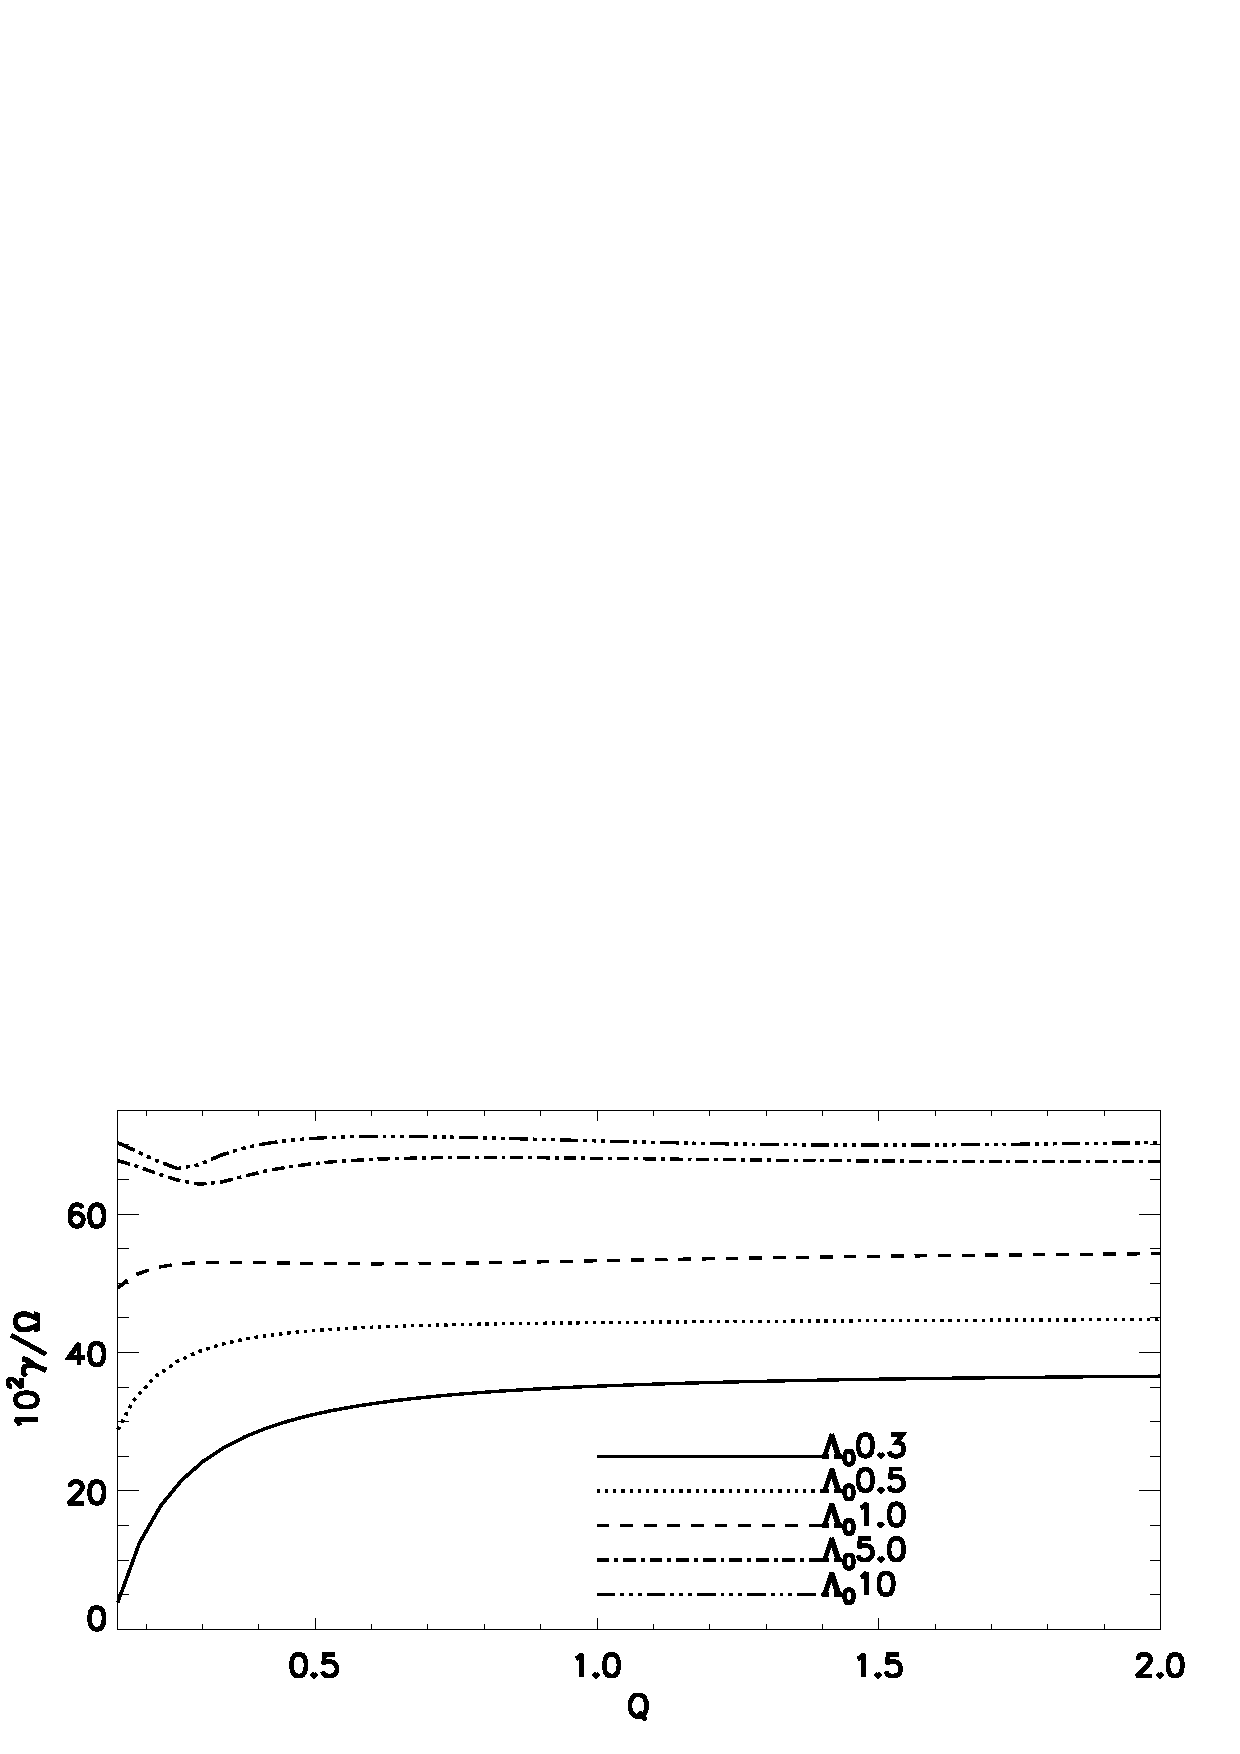
\includegraphics[width=\linewidth]{figures/compare_growth_poly_uniresis2}
  \caption{MRI growth rates as a function of $Q$ and midplane 
    Elsasser numbers, in polytropic disks with $\beta=100$ and uniform
    resistivity.  
    \label{compare_growth_poly_uniresis}}
\end{figure}

\cite{sano99} found that for MRI to operate, its 
wavelength $\lambda$ should fit inside the disk. That is,   
\begin{align}\label{sano_crit}
  \lambda \equiv
  \mathrm{max}\left(\lambda_\mathrm{ideal},\lambda_\mathrm{resis}\right)\lesssim
  2H, 
\end{align}
where the MRI wavelengths are given by 
\begin{align}\label{lambda_ideal}
  \frac{\lambda_\mathrm{ideal}}{2H} = \frac{4\pi}{\sqrt{15}} f \hat{v}_A =
  \frac{4\pi f}{\sqrt{15\beta\hat{\rho}}}
\end{align}
for ideal MHD, and 
\begin{align}\label{lambda_resis}
  \frac{\lambda_\mathrm{resis}}{2H} = \frac{2\pi}{\sqrt{3}}\frac{\hat{\eta}}{\hat{v}_A f} =
  \frac{2\pi f}{\Lambda_0}\sqrt{\frac{\hat{\rho}}{3\beta}} 
\end{align}
in the limit of high resistivity.  
   
Because $\hat{\rho}$ is weakly dependent
on $Q$ (Fig. \ref{eqm_den}), self-gravity only affects the
MRI through the factor $f$, which increases with decreasing $Q$ (see
Fig. \ref{plot_fq} in Appendix \ref{appen1}).   
This implies that sufficiently strong self-gravity can stabilize the
MRI by making $ 2H<\lambda $.   
 
In the ideal limit, we find $\lambda < 2H$ throughout most of the disk
for the values of $Q$ considered, so self-gravity does not affect
growth rates significantly. However, the ratio $\lambda/2H$ does
increase with stronger self-gravity. Consequently, the wavelength of
the instability, in units of $H$, increases. This is shown in
Fig. \ref{compare_result_lambda10} which plots the magnetic energies
for $\Lambda_0=10$ and a range of $Q$ values. The number of vertical
nodes decrease with $Q$, i.e. the disk accommodates fewer wavelengths
because increasing vertical self-gravity makes it thinner. 

\begin{figure}
  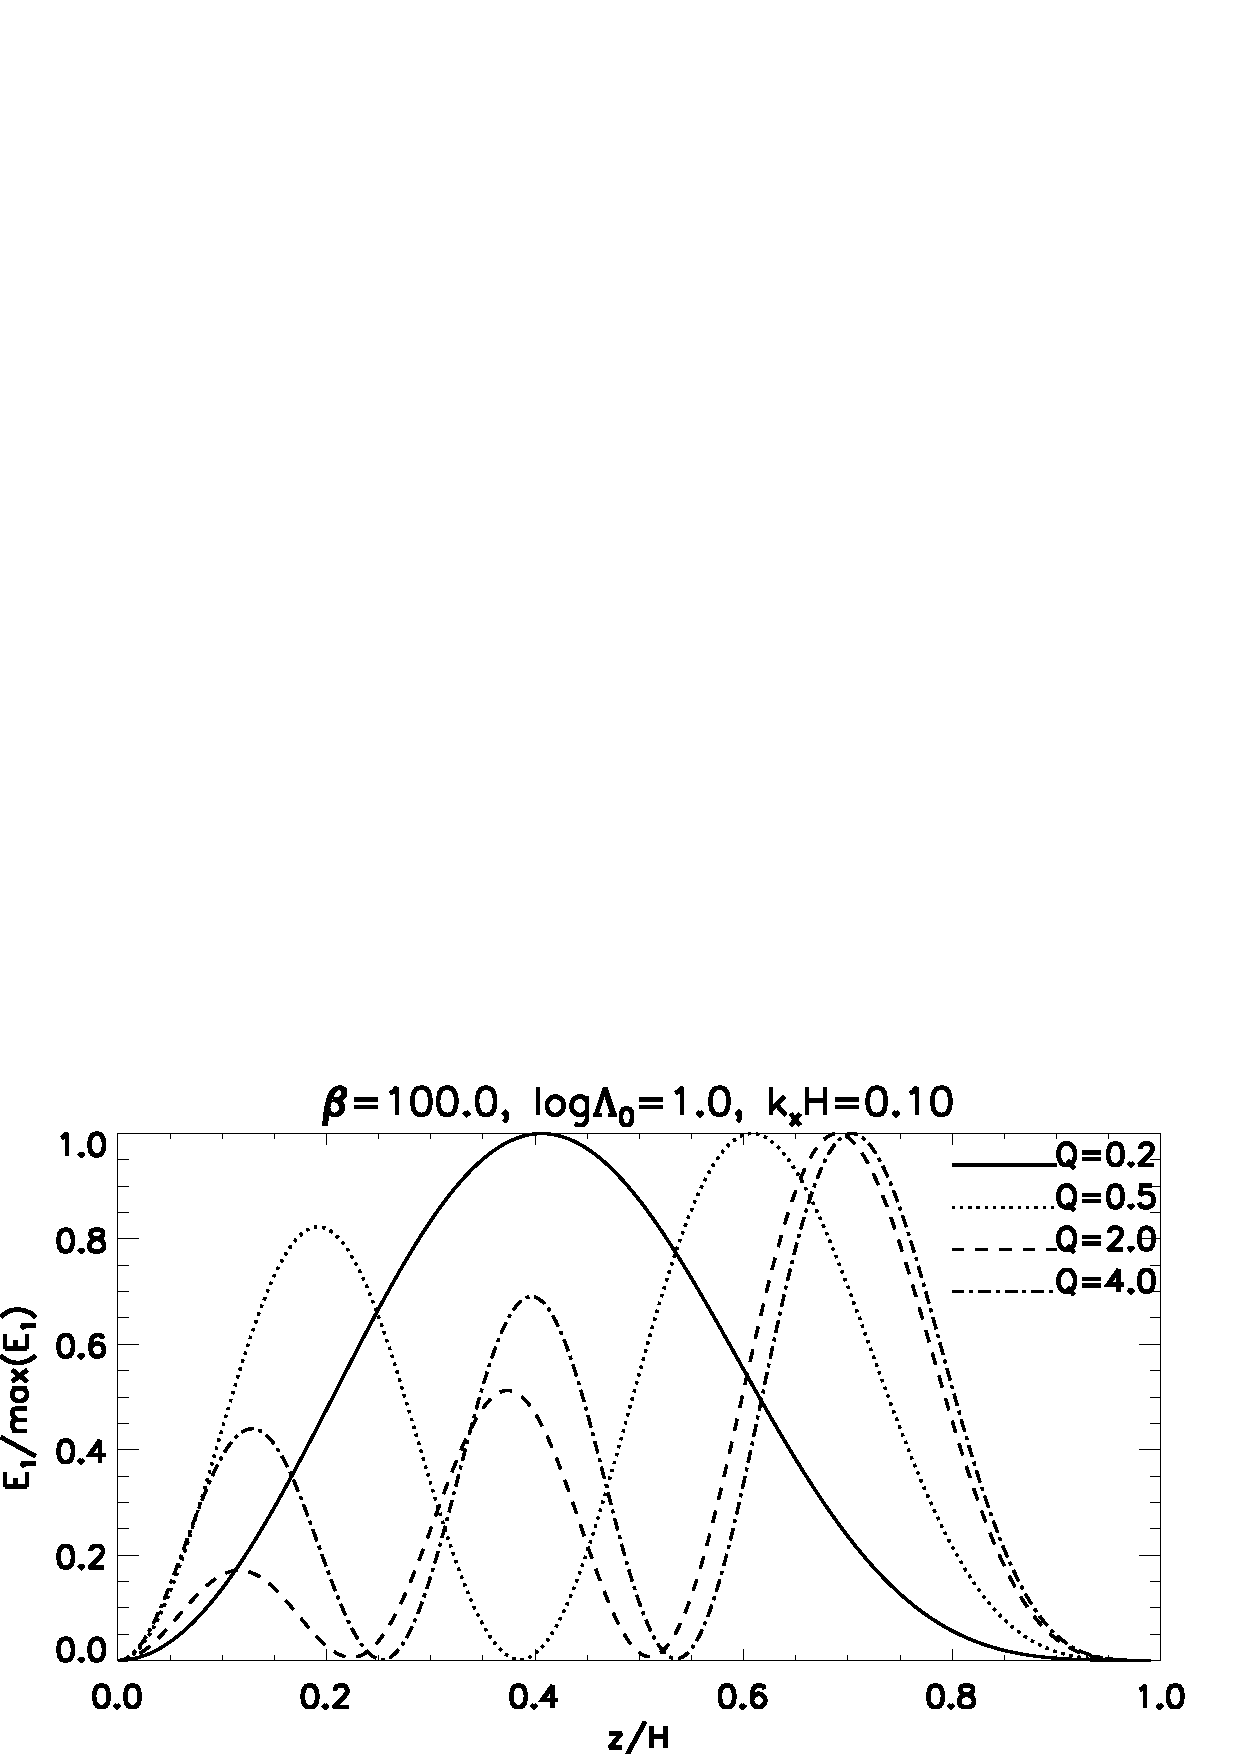
\includegraphics[width=\linewidth]{figures/compare_result_lambda10}
  \caption{MRI magnetic energies in ideal polytropic disks
    for different strengths of self-gravity.    
    \label{compare_result_lambda10}}
\end{figure}


Self-gravity appreciably decreases the MRI growth rates in the
resistive limit. Fig. \ref{lambda_poly_resis} plots 
Eq. \ref{sano_crit} for $\Lambda_0=0.3$. In the non-self-gravitating
disk ($Q=4$) the instability criterion is marginally satisfied and the
MRI operates. As $Q$ decreases, 
Eq. \ref{sano_crit} is violated and the MRI growth rate is
significantly reduced. This is seen for $Q=0.2$ where $\lambda \geq 2H$ throughout
the disk. (The instability is not suppressed since
Eq. \ref{lambda_ideal}---\ref{lambda_resis} is only exact for
unstratified disks.) Although the function 
$f(Q)$ does not change significantly for the range of $Q$ considered,
the dependence of $\lambda_\mathrm{resis}$ on $f(Q)$ is amplified by the
denominator $\Lambda_0<1$ in the resistive case. Modes in
Fig. \ref{lambda_poly_resis} have no nodes in the magnetic energy
$E_m$ except at $z\simeq0,\,H$, i.e. only the longest wavelength survives
with large resistivity. 
%self-gravity tips it over    

\begin{figure}
  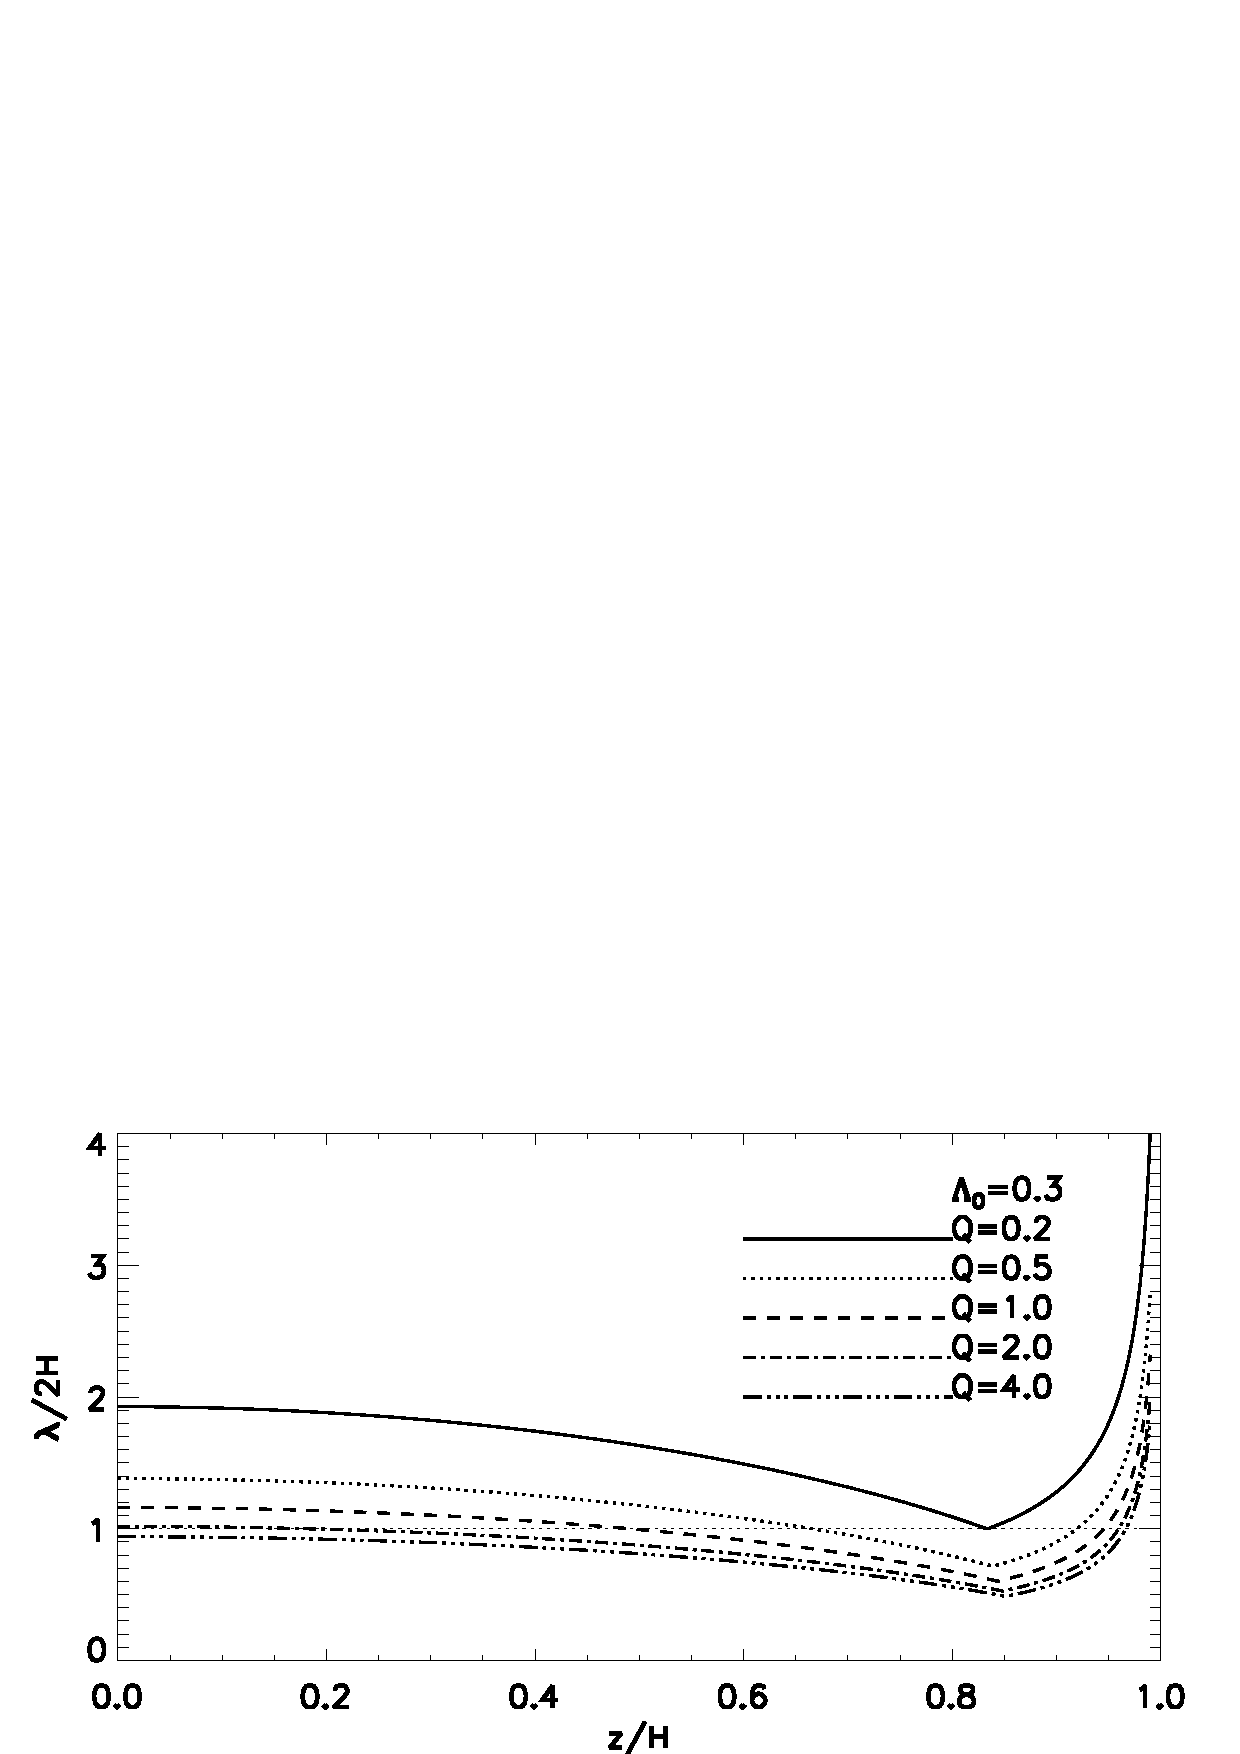
\includegraphics[width=\linewidth]{figures/lambda_poly_uniresis}
  \caption{Approximate wavelengths of the most unstable MRI modes as given by
    Eq. \ref{sano_crit}---\ref{lambda_resis}, normalized by the 
    disk thickness, as a function of height. MRI is expected to
    operate if $\lambda/2H\lesssim 1$. 
    \label{lambda_poly_resis}}
\end{figure}



\subsubsection{Layered 
  resistivity} 
Here we consider disks with midplane Elsasser number $\Lambda_0=0.1$
and a variable resistivity profile with
$A=10^2$. Fig. \ref{poly_layer} compares the magnetic  
energies for $Q=0.2,\,1$ and $4$. They have similar growth rates, $\gamma/\Omega
= 0.53,\,0.64$ and $0.66$, respectively. In the non-self-gravitating
limit ($Q=4$), the MRI is effectively suppressed for
$z\lesssim0.5H$. This is consistent with the picture of layered
accretion proposed for non-self-gravitating disks \citep{gammie96,fleming03}. 
However,in the massive disk ($Q=0.2$) the mode occupies a wider vertical
extent because its wavelength (in units of $H$) is larger. This
suggests that in massive disks, the MRI is not well localized to a
sub-layer within the height, even when the resistivity has a layered
structure.  


\begin{figure}
  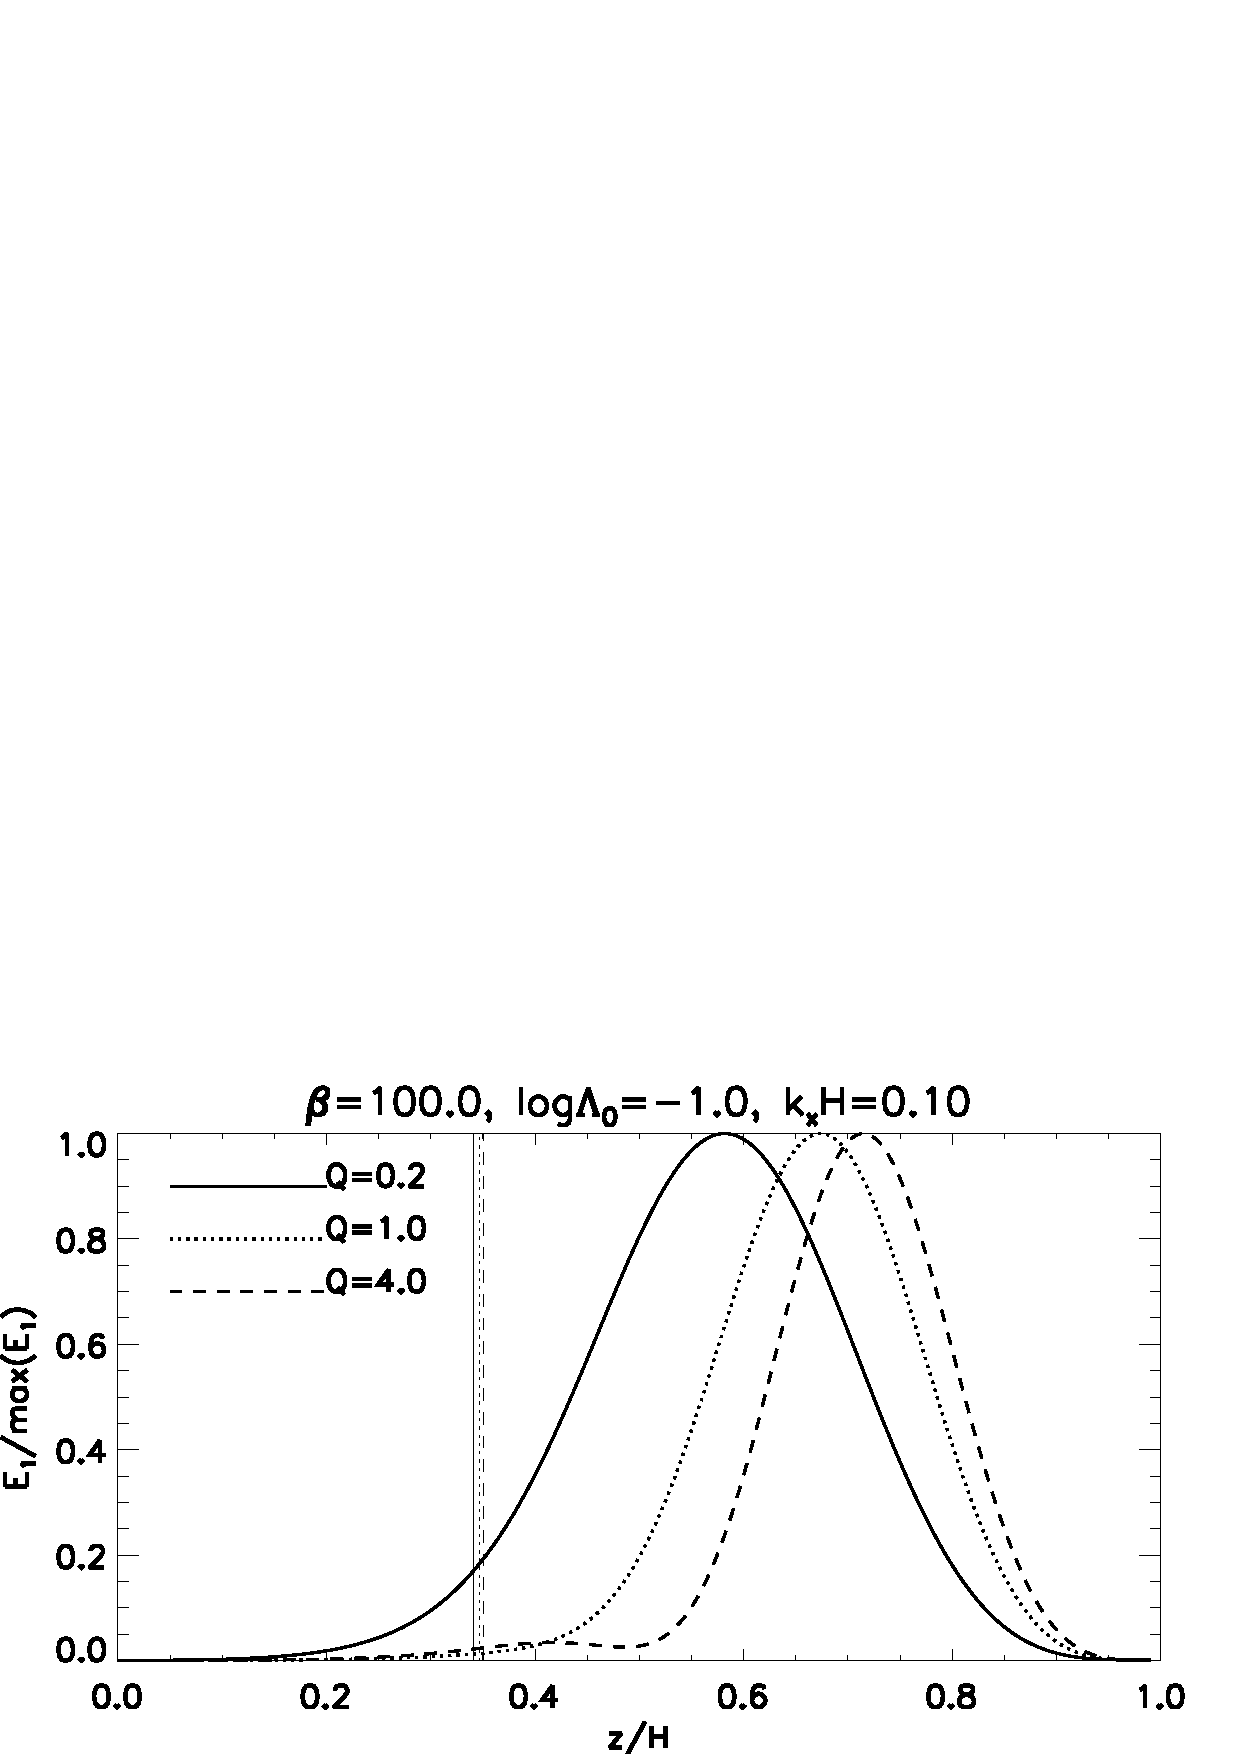
\includegraphics[width=\linewidth]{figures/compare_results_poly_layer_amp100}
  \caption{Magnetic energies as a function of height, for polytropic disks
    in which the conductivity increases by a
    factor $A=10^2$ in going from the midplane to the upper disk
    boundary. The vertical lines indicate $\Lambda=1$ for each value 
    of $Q$.
    \label{poly_layer}}
\end{figure}

\subsubsection{Dependence on $k_x$}
The above experiments show that with increasing 
disk self-gravity, the MRI becomes more global in the vertical
direction. We find a similar result in the horizontal direction. 
Fig. \ref{compare_growth_poly_kx} show MRI growth rates as a
function of $k_x$ for a range of $Q$ values. Increasing self-gravity
decreases the cut-off radial wavenumber for the MRI. We checked
that these modes have negligible density perturbations. Then we can 
understand this result by invoking the instability criteria for  
incompressible MRI in an unstratified Keplerian disk,
\begin{align}
  v_A^2(k_z^2 + k_x^2) < 3\Omega^2,
\end{align}
where $k_z$ is a vertical wavenumber \citep{kim00}. Setting $k_z^2\sim
\Omega^2/v_A^2$ and non-dimensionalizing, we find
\begin{align} 
  k_xH \lesssim \frac{\sqrt{\beta}}{f},
\end{align}
where order-unity factors have been dropped. Despite a simplistic
approach, this demonstrates that with increasing self-gravity
(increasing $f$), we expect MRI modes with small radial
length scales to be suppressed.   


 
\begin{figure}
  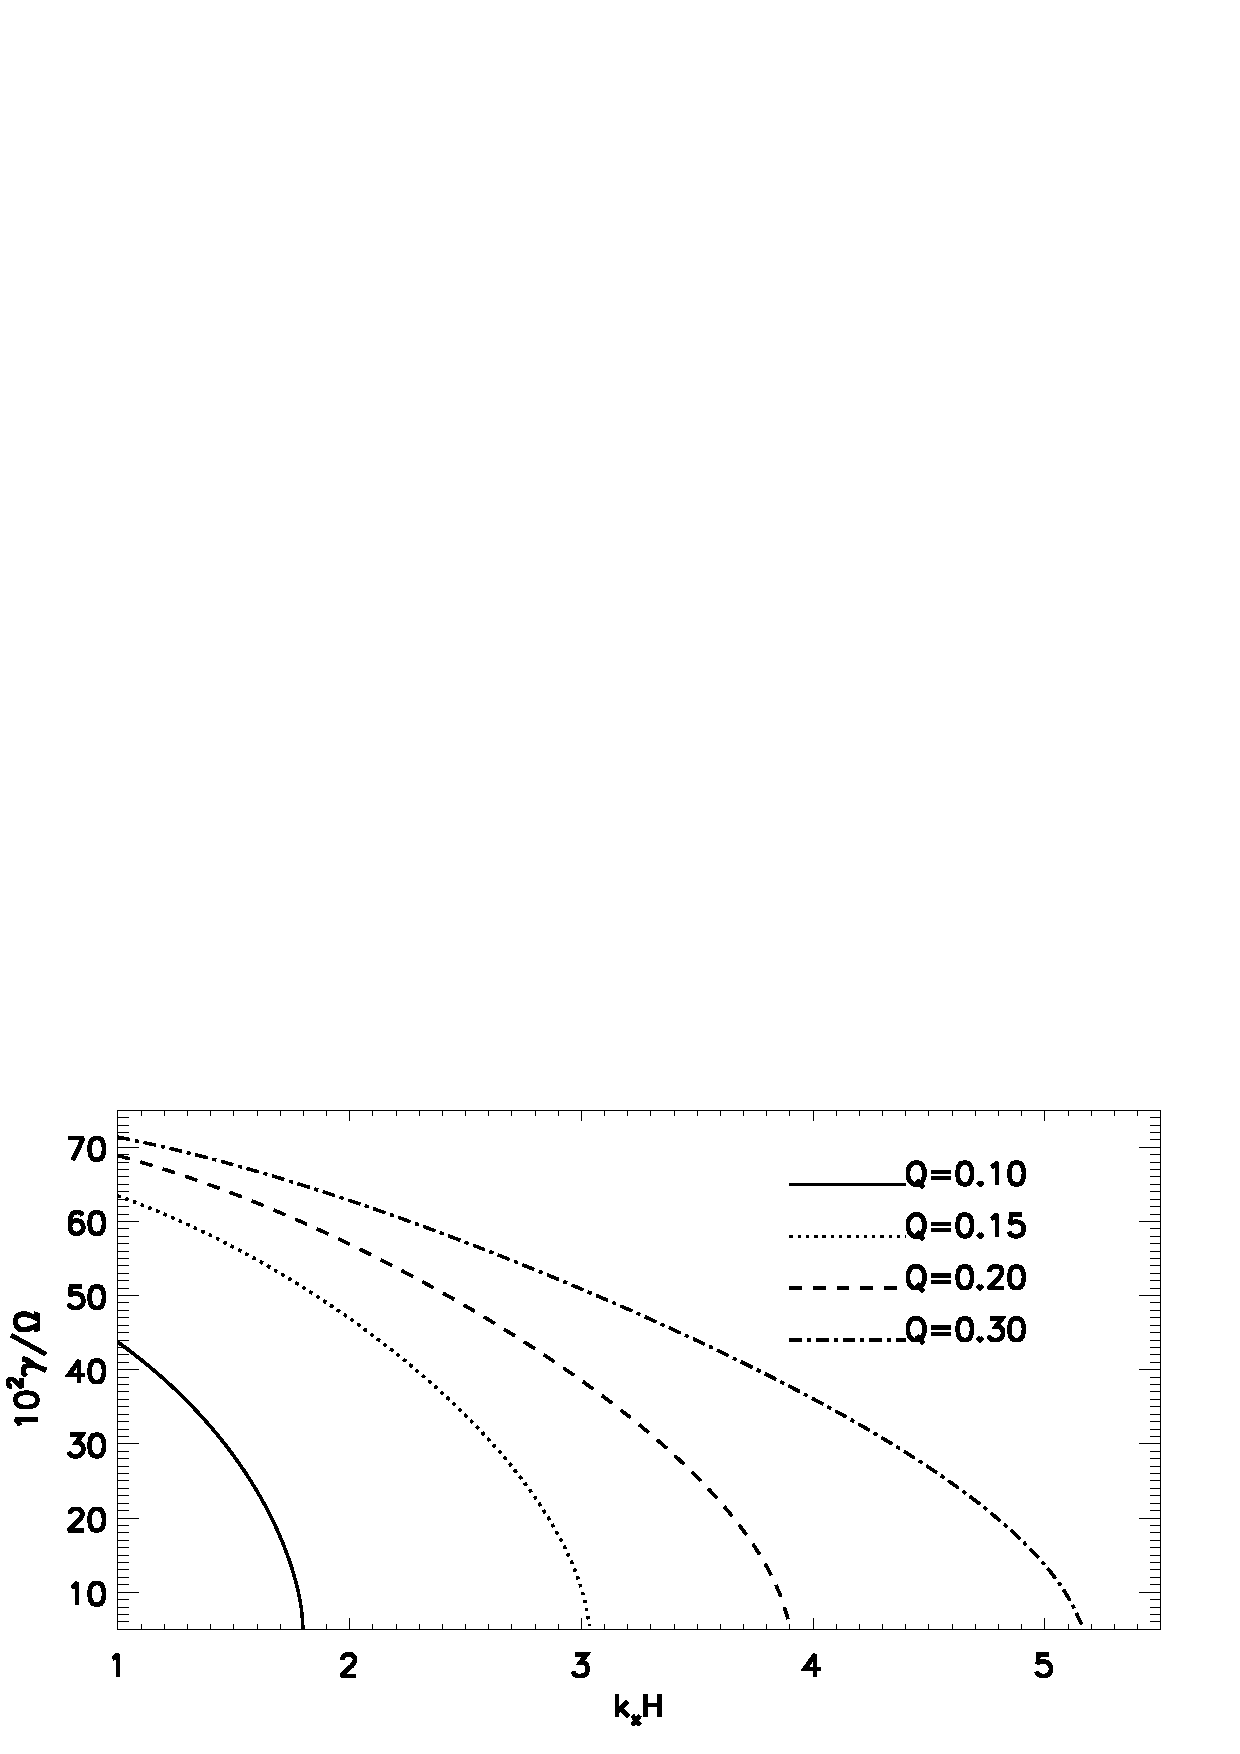
\includegraphics[width=\linewidth]{figures/compare_growth_poly_varQ_kx}
  \caption{MRI growth rates in self-gravitating polytropic disks, as a
    function of the horizontal wavenumber $k_x$. The disk is ideal
    ($\Lambda_0=10^2,\, A=1$) with $\beta = 40$. These modes have negligible
    density/potential perturbations.  
    \label{compare_growth_poly_kx}}
\end{figure}



\subsection{Influence of self-gravity on the MRI through the linear
  response}  
Our goal here is to examine whether or not self-gravity can amplify
the density perturbations associated with the MRI. We compute unstable modes
in a massive isothermal disk with $Q=0.2$ (corresponding to
$Q_\mathrm{2D}=0.72$), which is still expected to be marginally  
stable to gravitational instability \citep[][who find
a critical value of  $Q\simeq 0.2$]{mamat10}.   
The upper disk boundary is set to $Z_s=H$. 

%resolution Nz=256

\subsubsection{Ideal disks}
We first consider ideal MHD by adopting a uniform 
resistivity with $\Lambda_0=100$.  
Fig. \ref{gravity_energy} plots MRI growth rates as a function of
$k_x$ for several values of $\beta$. The curves are color-coded 
according $\tau$. (Recall $\tau\to1$ implies self-gravity dominates
over magnetic perturbations, and $\tau\to0$ is the opposite limit.)  
The potential perturbation is negligible for all cases when
$k_xH\lesssim 0.5$, since the MRI becomes incompressible as $k_x\to
0$.  

\begin{figure}
  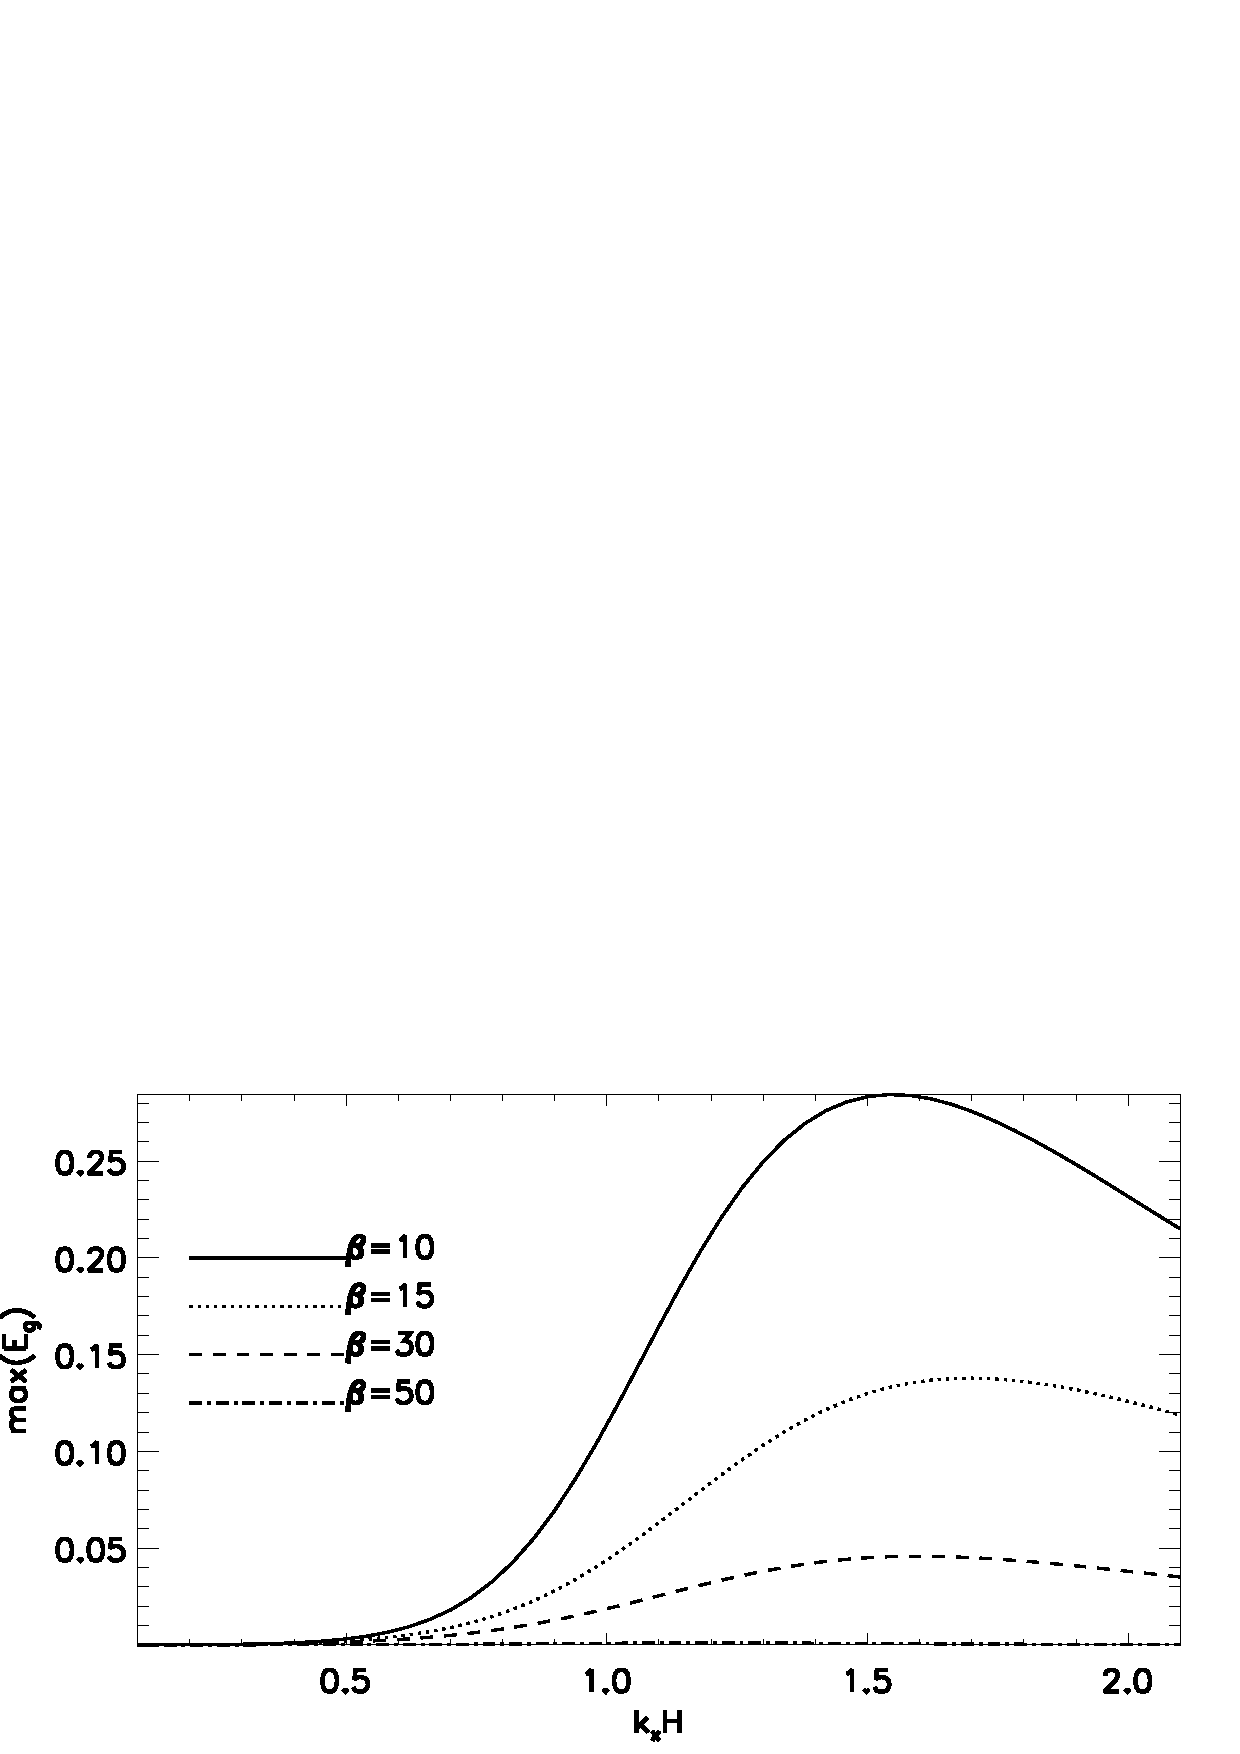
\includegraphics[width=\linewidth]{figures/compare_energy_ideal}
  \caption{Growth rates of MRI modes in isothermal self-gravitating
    disks with $Q=0.2$ ($Q_\mathrm{2D}=0.72$) in the limit of ideal MHD
    ($\Lambda_0=10^2$, $A=1$), for a range of field strengths $\beta$. The
    colorbar measures the importance of self-gravity by $\tau$.  
    %{\bf ADD BETA=8}
    \label{gravity_energy}}
\end{figure}

For $\beta\gg 1$, i.e. a weak field, density perturbations are
negligible and the incompressible MRI operates. However, as $\beta$ is
lowered and the MRI growth rate reduced, we find non-negligible
potential perturbation for $k_xH=O(1)$. This suggests that in a
strongly magnetized disk that still permits the MRI, the associated
density perturbation can be important when the disk is
self-gravitating. %but formall stable 



\subsubsection{Resistive disks}
We repeat the above calculation for resistive disks, but fix
$\beta=100$ and vary the midplane Elsasser number $\Lambda_0$. Growth
rates are shown in Fig. \ref{gravity_energy_resis}. 
Interestingly, the highly resistive case $\Lambda_0=0.1$ has
comparable magnetic and gravitational energies: at $k_xH\simeq1.3$ we
find $\tau\sim 0.3$, which corresponds to $\avg{E_g}\sim 0.5\avg{E_m}$.  
Fig. \ref{mri_massive_cowling} compares the magnetic
energy of this mode to that computed in the \emph{Cowling  
  approximation}, where the Poisson equation is ignored in the 
linearized equations and the potential perturbation set to zero  
(formally letting $Q\to\infty$ in Eq. \ref{lin_poisson}).  
The growth rate increases when self-gravity is included in the linear
response, since self-gravity is usually destabilizing. However, 
$\gamma$ and $E_m$ are very similar, indicating that the instability
in the self-gravitating calculation is fundamentally still the MRI.   

\begin{figure}
  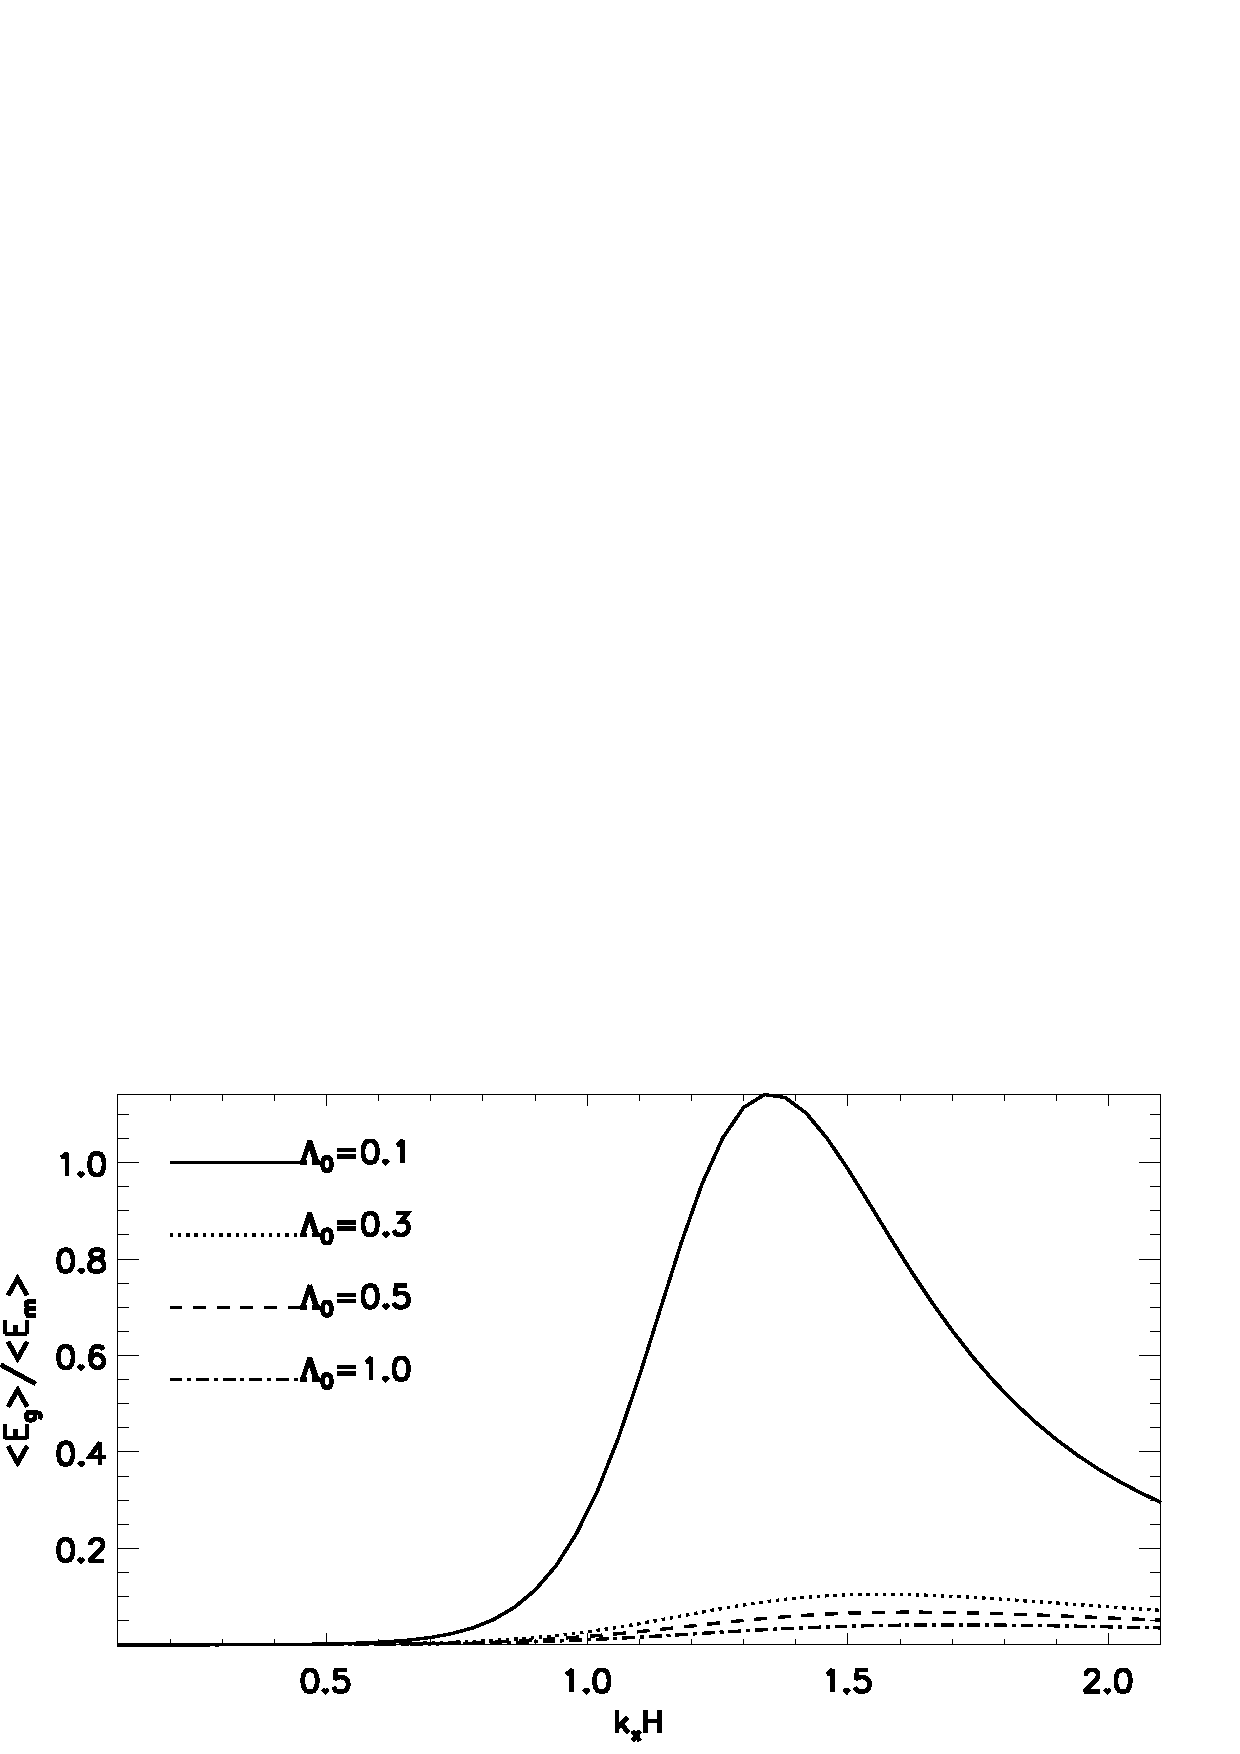
\includegraphics[width=\linewidth]{figures/compare_energy_resis}
  \caption{
    Growth rates of MRI modes in an isothermal self-gravitating
    disk with $Q=0.2$ ($Q_\mathrm{2D}=0.72$) at fixed $\beta=100$, 
    for a range of midplane Elsasser numbers. The resistivity is
    uniform. The colorbar measures the importance of self-gravity by $\tau$. 
    \label{gravity_energy_resis}}
\end{figure}


\begin{figure}
  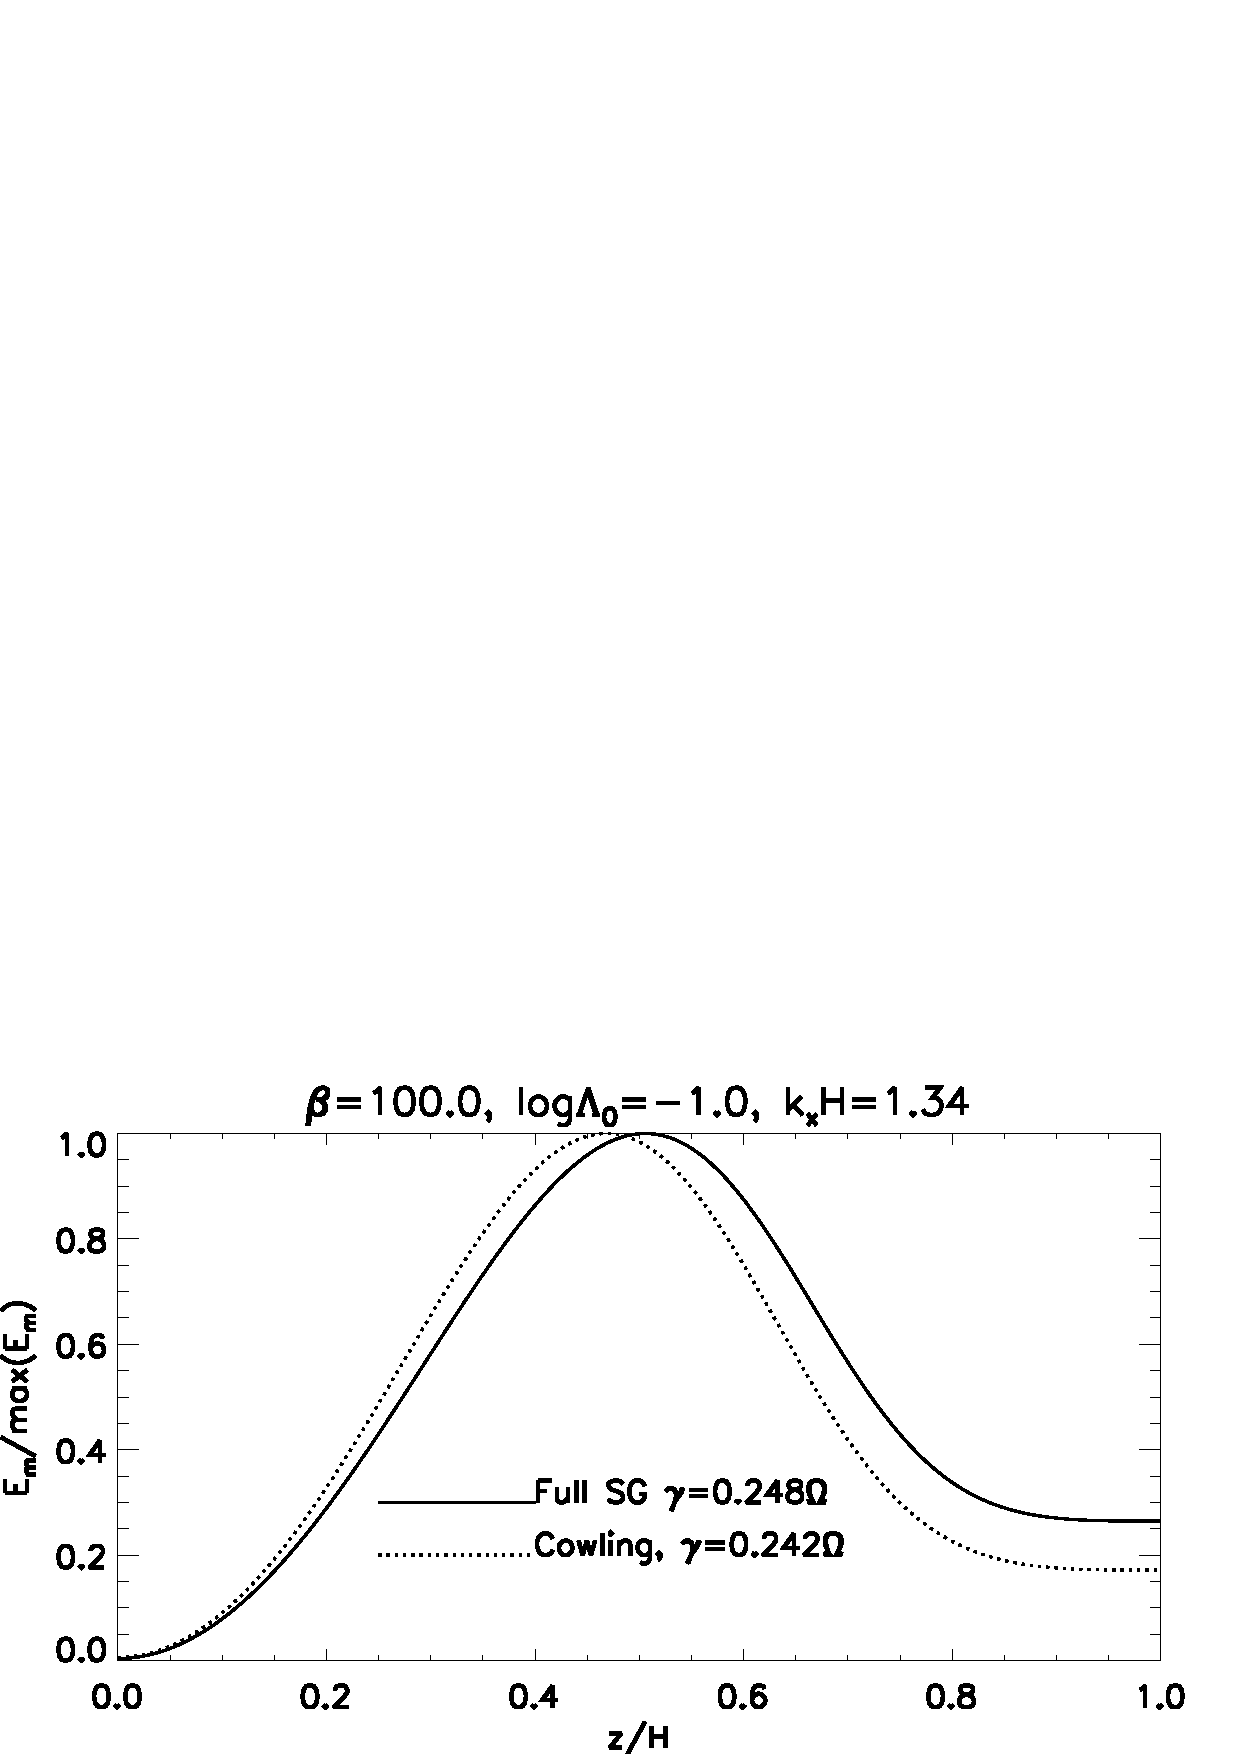
\includegraphics[width=\linewidth]{figures/compare_result_cowling}
  \caption{Magnetic energy associated with the linear mode with
    largest gravitational-to-magnetic energy ratio in 
    Fig. \ref{gravity_energy_resis} (solid) compared with that computed
    under the Cowling approximation (dotted). %{\bf REDO FIGURE}
    \label{mri_massive_cowling}}
\end{figure}

Fig. \ref{mri_massive_resis} plots the energies associated with the 
MRI mode discussed above. 
The gravitational energy exceeds the 
magnetic energy near the midplane ($z\lesssim0.2H$). The growth rate
$\gamma=0.25\Omega$ is not much smaller than that of the most unstable
mode ($\gamma=0.36\Omega$ for $k_xH=0.1$), so significant density
perturbations will grow on dynamical timescales for this
system, even though GI is not expected.

\begin{figure}
  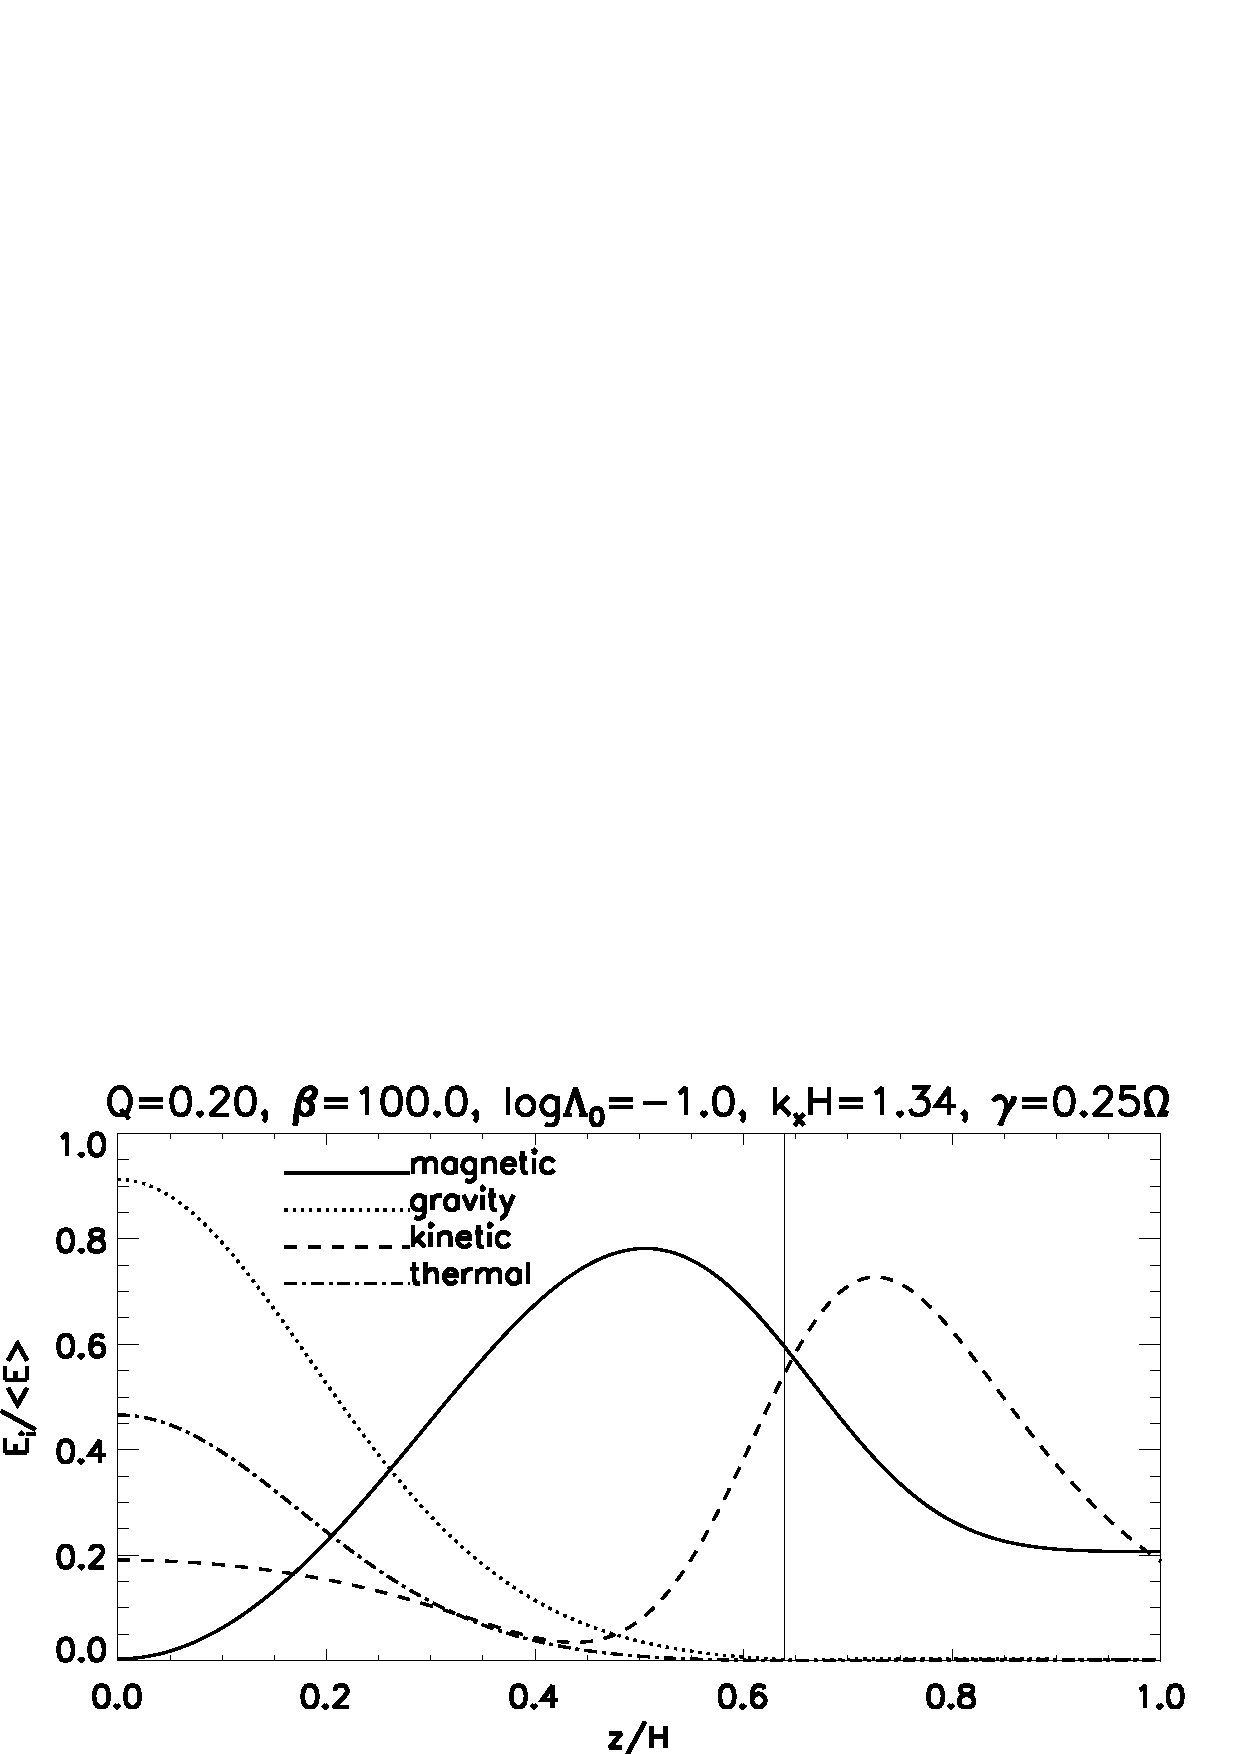
\includegraphics[width=\linewidth]{figures/result_resis_sg}
  \caption{Example of a resistive MRI mode with significant
    gravitational potential perturbation. The disk is isothermal. 
    The vertical line
    indicates $\Lambda=1$.  
    \label{mri_massive_resis}}
\end{figure}

\subsubsection{Qualitative interpretation} 
To make sense of the above results, we first return to ideal MHD and 
consider regions close to the disk midplane ($z\sim 0$), where
self-gravity is expected to be most important. For this discussion we
will ignore stratification and set $d^2/dz^2\to -k_z^2$. The governing
equations are then 

\begin{align}
  &  0= v_A^2k^2\dvx + \imgi\sigma\left(\imgi\sigma \dvx - 2\Omega\dvy + \imgi k_x \w\right),\label{simp1}\\
  &  0= v_A^2k_z^2\left(\dvy + \frac{\imgi S
  }{\sigma}\dvx\right) + \imgi\sigma\left(\imgi\sigma\dvy +
  \frac{\kappa^2}{2\Omega}\dvx\right),\label{simp2}\\
  & 0 = -k_z^2\w + \frac{\sigma^2}{c_s^2}W + \sigma k_x \dvx, \label{simp3}\\
  & 0 = k^2\dphi + \frac{\Omega^2}{c_s^2Q}W,\label{simp4}
\end{align}
where $k^2 = k_z^2 + k_x^2$. We imagine an iterative procedure to
solve the above equations, starting from the Cowling approximation
where $\delta\Phi\to0$ and $Q\to\infty$. This is the standard MRI and we denote the
solution as $\dvx^{(0)}$, $\dvy^{(0)}$ and $W^{(0)}$. Eq. \ref{simp3} implies
\begin{align}
  W^{(0)} = \frac{c_s^2\sigma k_x \dvx^{(0)}}{c_s^2k_z^2 - \sigma^2}. 
\end{align}
We argue below that $c_s^2k_z^2\gg \sigma^2$ by taking $k_z\sim
\Omega/v_A$. Then, recalling $W=c_s^2\delta\rho/\rho$, we can write
\begin{align}
  \frac{\delta\rho^{(0)}}{\rho} \sim
  \frac{\sigma}{\Omega}\frac{1}{\beta}\left[\frac{k_x\dvx^{(0)}}{\Omega}\right].   
\end{align}
The MRI has, in general, a non-zero density perturbation. However, it
is negligible for $k_x\to 0$ and/or a weak field ($\beta \gg 1$). 

% In general, the
%compressible MRI has $W^{(0)}\neq0$, since

We now include self-gravity.  The Poisson equation implies $W^{(0)}$
has an associated potential perturbation,     
\begin{align} 
  \dphi = -\frac{\Omega^2}{c_s^2 Q k^2} W^{(0)}.
\end{align}
Physically, we expect $k^2\geq0$, so that a positive (negative) local density
perturbation causes a negative (positive) local potential
perturbation. We then insert $\dphi$ back into the momentum and
continuity equations, and ask how does this potential perturbation
modify the Cowling solution? Writing $\dvx^{(0)} \to \dvx^{(0)} +
\dvx^{(1)}$ and similarly for $\dvy $ and $ W$, we find 


\begin{align}
  &   k_x\sigma \dphi = v_A^2k^2\dvx^{(1)} + \imgi\sigma\left[\imgi\sigma
  \dvx^{(1)} - 2\Omega\dvy^{(1)} + \imgi k_x W^{(1)}\right], \label{simp_pert1}\\ 
  &  0= v_A^2k_z^2\left[\dvy^{(1)} + \frac{\imgi S
    }{\sigma}\dvx^{(1)}\right] + \imgi\sigma\left[\imgi\sigma\dvy^{(1)} +
  \frac{\kappa^2}{2\Omega}\dvx^{(1)}\right],\label{simp_pert2}\\
  & k_z^2\dphi  = \left(\frac{\sigma^2}{c_s^2}-k_z^2\right)W^{(1)} +
  \sigma k_x \dvx^{(1)}.\label{simp_pert3} 
\end{align}
Now, if the perturbations to the magnetic field remain
unchanged, i.e. the mode remains close to the standard MRI as observed
in Fig. \ref{mri_massive_cowling}, then $\dvx^{(1)} \sim 0$ and
$\dvy^{(1)}\sim0$, so Eq. \ref{simp_pert2} is 
satisfied. Eq. \ref{simp_pert1} then require $\dphi +
W^{(1)}\sim0$. This is compatible with Eq. \ref{simp_pert3} if 
\begin{align}
  \left|k_z^2\right| \gg \left|\frac{\sigma^2}{c_s^2}\right|. \label{cond}
\end{align}
For the ideal MRI,  we take $k_z\sim \Omega/v_A$. Then
$|\sigma^2/c_s^2k_z^2|\sim |\sigma^2/\Omega^2\beta|\ll1$ because
$|\sigma|\lesssim \Omega$ and we are considering $\beta\gtrsim 10$. 
Thus Eq. \ref{cond} is generally satisfied.   

The above assumptions imply
\begin{align}
  W^{(1)} \sim \frac{\Omega^2}{c_s^2 Q k^2} W^{(0)},\label{feedback}
\end{align} 
which indicates a non-zero density perturbation due to the
MRI can be amplified by self-gravity. Now, for $k_xH\sim 1$ we have
$|k_z^2/k_x^2|\sim \beta/f^2\gg1$ because $f=O(1)$ and $\beta\gtrsim10$
for the cases considered above. Then
\begin{align}
  \left|\frac{W^{(1)}}{W^{(0)}}\right| \sim \frac{1}{Q\beta}, 
\end{align}
 suggesting stronger amplification of the density field by 
 self-gravity with increasing field strength (decreasing
 $\beta$). 

 

 The above arguments can be adapted to the resistive
 disk. Eq. \ref{simp3}---\ref{simp4} are unchanged, while resistive
 terms appearing in Eq. \ref{simp1}---\ref{simp2} only involve the
 potential perturbation through $\w$. For the resistive MRI we take
 $k_z\sim v_A/\eta$ and $|\sigma|\sim v_A^2/\eta = \Lambda\Omega$
 \citep{sano99}. Then $|\sigma^2/c_s^2k_z^2|\sim 1/\beta \ll 1$ so
 Eq. \ref{cond} is satisfied. Noting that $k_z^2\sim
 \Lambda^2\Omega^2\beta/c_s^2$, the feedback equation becomes
 \begin{align}
   \left|\frac{W^{(1)}}{W^{(0)}}\right| \sim
   \frac{1}{Q\left(f^2\hat{k}_x^2 + \beta\Lambda^2\right)},
 \end{align}
 so increasing the resistivity (decreasing $\Lambda$) should enhance
 density perturbations.  

%these arguments assume, of course, there is a non-zero density
%perturbation in the first place for self-gravity to ehance. 

 For weak fields in an ideal disk, the MRI has a vertical
 wavelength $\lambda \ll H$. It will be almost incompressible so the 
 `seed' density perturbation $W^{(0)}$ is small.  
 The perturbed mass contained within 
 $\sim \lambda$ is small and its potential is
 unimportant. Furthermore, considering the stratified  
 disk, $\lambda\ll H$ imply rapid variations in the density
 perturbation across the disk height, averaging to zero, so the
 magnitude of the associated potential perturbation is small. 
 Self-gravity does not affect the MRI in this regime.   
 
%the `seed' density pert is also small
%weak amplification

 However, a strong field and/or large resistivity increases the MRI
 vertical wavelength. When the vertical scale of the MRI becomes
 comparable to the disk thickness, i.e. $\lambda\sim H$, the
 perturbed mass across the disk height can contribute to a net potential
 perturbation. We therefore expect a necessary condition for
 self-gravity to affect the MRI is for the latter to be weak. 
%we are not considering GI yet

%Our
% interpretation above also assumes that the Cowling solution can
% provide some `seed' density perturbation. 
%Thus we also require the
% MRI to be compressible. 
%there has to be some  `seed' density perturbation provided by the
%non-SG MRI 

%\section{Isothermal limit}\label{isothermal}
We now examine the limit $\Gamma\to 1$, where the unperturbed disk becomes isothermal
, but perturbations are evolved with an adiabatic index
$\gamma=1.4$. We consider a nearly-isothermal polytropic background
and strictly isothermal backgrounds. These cases are treated
separately because the equilibrium structures have different
functional forms. A comparison between them provide another
check on our numerical results. 

\subsection{Large polytropic index}
We first consider setting $n=10$ to produce an almost radially
isothermal equilibrium with $p\propto \rho^{1.1}$. This allows us to use the
numerical code as set up for polytropic equilibria without
modification. We also adopt $A=2.5$ and $h=0.25$ for reasons given
in \S\ref{varpolyn}. The relatively large aspect-ratio does not
violate the thin-disk approximation as large $n$ implies the 
density decays rapidly away from the midplane. Also because of this,
we set the upper disk boundary at $Z_s=0.6$ to avoid very low 
densities. %All other parameters are the same as before. 

%3d-ness of core is 0.55
%3d-ness averaged over 0.9, 1.1 is 0.37
%%  Despite the larger
%% value of $\gamma/\Gamma$ than case 8 (see Table \ref{linsims}), the flow
%% three-dimensinality is the same.   

For this setup we obtained $\omega/m\Omega_0=0.9883$,
$\nu/\Omega_0=0.1375$ and $\avg{\theta_m}=0.35$. The top panel of
Fig. \ref{polyn10} shows the meridional flow at the vortex core. The
vortical motion is distinct and more apparent than case 3a, despite
the smaller value of $\gamma/\Gamma$ in the present case. 
However, apart from this difference, the solution is qualitatively
similar to case 3a.   

\begin{figure}[!t]
  \centering
  %% \includegraphics[scale=.425,clip=true,trim=0cm 1.cm 0cm
  %%   0cm]{figures/n10.0_gmma1.4_wq_3d_real_zslices.ps}
  \includegraphics[scale=.425,clip=true,trim=0cm 1.83cm 0cm
    0.25cm]{figures/n10.0_gmma1.4_vel3d_rz_dvz_nofill.ps}
   \includegraphics[scale=.425,clip=true,trim=0cm 0cm 0cm
    0.25cm]{figures/iso_vel3d_rz_dvz_nofill.ps}
  \caption{Perturbed meridional flow at $\phi=\phi_0$ for a $n=10$
    polytropic disk equilibrium (top) and a strictly isothermal
    equilibrium (bottom). 
    \label{polyn10}}
\end{figure}



\subsection{Strictly isothermal equilibrium}
%Because we have formulated the linear problem in terms of entropy and
%pressure length-scales, in order to calculate the RWI for strictly
%isothermal disks, we can just replace 
Modifications to our standard setup are required to treat  
disk equilibria with $p=\ciso^2\rho$ ($\Gamma\equiv 1$), where 
the constant sound speed $\ciso=\Hiso\Omega_k$, $\Hiso=\hiso
r_0(r/r_0)^{3/2}$ is the isothermal scale-height, and $\hiso$ is the
characteristic aspect-ratio at $r_0$. 
%We set $\ciso=\Hiso
%\Omega_k$, where $\Hiso\propto r^{3/2}$ is the isothermal scale-height
%and we define $\hiso=\Hiso/r_0$. 
The dimensionless vertical 
co-ordinate is now $Z=z/\Hiso$. The isothermal atmosphere is
exponential, $g(Z)=\exp{(-Z^2/2)}$, so there is no surface. In
practice we choose a finite vertical domain, i.e. $Z=Z_s$ represents a
constant number of isothermal scale-heights above the midplane. 

In the linear code we simply replace expressions for the entropy
and pressure length-scales by those corresponding to the isothermal
disk: the function $H\to\Hiso$ and $g(Z)$ becomes the Gaussian above. 
%% We set parameter values to mimic the large-$n$ polytrope in the 
%% previous section:  $Z_s=3$ and $\hiso=0.05$,
%% so that for both setups the pressure is reduced by roughly the 
%% same factor in going from the midplane to the upper boundary, and the
%% midplane temperature is roughly equal at $r_0$. 
{\bf
We choose $Z_s=3$ and $\hiso=0.05$, so the isothermal disk has roughly
the same temperature as that in the midplane of the large-$n$ 
polytrope considered above (at $r_0$).} In going from the
midplane to the upper boundary, the density is also reduced by
approximately the same factor for both cases.  


We obtain $\omega/m\Omega_0=0.9860$, $\nu/\Omega_0=0.1008$ and
$\avg{\theta_m}=0.39$. The perturbations plotted in
Fig. \ref{isothermal_case} are similar to case 3a, so we expect these
are features of the RWI in nonhomentropic flow, rather than
associated with the chosen parameter values. The perturbed meridional
flow shown in Fig. \ref{polyn10} (bottom panel) is in qualitative
agreement with the large-$n$ polytrope. 
The result is, however, quite different to
isothermal linear perturbations, for which \cite{meheut12} found the 
vertical velocity appears to have a node at $r_0$ ({\bf see their Fig. 3d where the vertical velocity changes sign across co-rotation radius}
, i.e. the fluid column is hydrostatic there). 
Note that both $\gamma/\Gamma$
and the growth rate are slightly smaller than the nonhomentropic case 3a,
but here the vortical motion is more prominent. 
%contribution from higher m?

\begin{figure}[!t]
  \centering
  \includegraphics[scale=.425,clip=true,trim=0cm 0.cm 0cm
    0cm]{figures/iso_wq_3d_real_zslices.ps}
  \caption{Pressure (top, $W$), density (middle, $Q$) and entropy
    (bottom, $S$) for a globally isothermal background. 
    \label{isothermal_case}}
\end{figure}

  Fig. \ref{polyn10_vz} shows the vertical 
  velocity at the vortex core as a function of height. The strictly
  isothermal background {\bf (thick solid)} has a slightly larger $\dd v_z$ than the
  large-$n$ polytrope {\bf (thick dashed)}. This is consistent 
  with previous findings that vertical motions oppose the RWI
  \citep{lin12c}, as the former case has a smaller growth rate than
  the latter. The {\bf thick lines are} qualitatively similar to case
  3a in Fig. \ref{compare_dvz}, but these are not directly comparable 
  because the present case differs in both the background structure and adiabatic index  to 
  those in Fig. \ref{compare_dvz}. 
  
  \begin{figure}[!t]
    \centering
    \includegraphics[scale=.425,clip=true,trim=0cm 0cm 0cm
      0.25cm]{figures/temp_dvz3}
    \caption{
      {\bf
        Vertical velocity as a function of $z$ at the vortex core
        $(r_0,\phi_0)$, for the $n=10$ 
        polytropic disk equilibrium (dashed) and a strictly isothermal
        equilibrium (solid) shown in 
        Fig. \ref{polyn10}, with free upper boundaries (thick lines). Corresponding thin 
        lines impose zero vertical velocity at $z=Z_s$ (growth rates increased by less than $0.5\%$ from the free boundary condition).
        Notice that changing upper disk boundary conditions only 
        affected the solution near $z=Z_s$ (cf. Fig. \ref{compare_dvz}). 
        This is consistent \cite{lin12c}, who found the
        influence of upper disk boundary condition to diminish with
        increasing polytropic index $n$. 
      }
      \label{polyn10_vz}}
\end{figure}
  
  Finally, we illustrate again a correlation 
  between meridional vortical flow and a tilted column of negative
  vertical vorticity perturbation in Fig. \ref{iso_vort3d_pz}. The figure is
  {\bf qualitatively} similar to that for polytropic backgrounds (case 3a in
  Fig. \ref{nonhomentropic_case_vort3d_pz}).{\bf  We find an average tilt
    of $1-~\avg{\cos{\theta}}_Z=0.0084
    \ll1$, so the vorticity column is nearly vertical.} 
  
  %% but the tilt magnitude
  %%   is larger for the isothermal background. 
  %Note that we chose
  %$r=1.03r_0$ as the radial slice, so that $\delta\omega_z <0$ along
  %the vertical line $(\phi_0,z)$. 
  %%  A plot for $r=1.02r_0$ also display
  %% the tilt, but in that case $\delta\omega_z$ was found to be positive
  %% at   
  

\begin{figure}[!t]
  \centering
  \includegraphics[scale=.425,clip=true,trim=0cm 0cm 0cm
    0.25cm]{figures/iso_vort3d_pz2.ps}
  \caption{
      Vertical vorticity perturbation, $\delta\omega_z$, in the
      $(\phi,z)$ plane at $r=1.03r_0$ for the strictly isothermal
      background. Regions of $\delta\omega\leq0$ are delineated by
      while lines. The center of meridional vortical motion identified
      in Fig. \ref{polyn10} occurs at height $z\sim
      H_\mathrm{iso}$. {\bf The azimuthal range
        $\phi-\phi_0\in[-0.5,0.5]\pi/m$ corresponds to anti-cyclonic
        motion about the vortex core.
        [ A plot for $r=1.02r_0$ also display
      tilted lines of constant $\delta\omega_z$, but in that case $\delta\omega_z > 0$
      at $(\phi_0, H_\mathrm{iso})$.]
      } 
    \label{iso_vort3d_pz}}
\end{figure}

\subsection{A nonlinear simulation}
%boundary conditions
%compare Q at different heights
%compare W in rz plane - vortical motion
We have also performed global 3D hydrodynamic simulations
using the \zeus  finite-difference code \citep{hays06}. As the focus
of this work is the linear problem, though, we defer a full discussion
of these nonlinear simulations to a follow-up paper. Our priority here
is to verify the  vortical motion in the meridional plane, which
appears characteristic in  the linear RWI solution for  nonhomentropic
flow.   

\subsubsection{Setup}
We use spherical polar co-ordinates $(\rsph,\theta,\phi)$ to describe
the disk, taken to be initially strictly isothermal as described above.  The
computational domain is $\rsph\in[0.2,2.0]r_0$,
$\theta\in[\theta_\mathrm{min},\pi/2]$, $\phi\in[0,2\pi]$ and is
divided into $(512,48,512)$ zones, with
$\tan{(\pi/2-\theta_\mathrm{min})}=3\hiso$ and $r_0=10$. 
The grid is logarithmically spaced in radius and uniformly spaced in 
the angular co-ordinates. Boundary conditions 
are outflow in $\rsph$, reflection in $\theta$ and periodic in $\phi$.  
Additional damping to meridional velocities near radial boundaries are
employed to reduce reflections \citep{valborro07}.  

%The disk is initially strictly isothermal as described in the previous section, and the vertical domain is such that 
%$\tan{(\pi/2-\theta_\mathrm{min})}=3\hiso$. 

After some experimentation, we found it was most convenient to start with a smooth disk.
In this case, a surface density $\Sigma\propto r^{-3/2}$, and tapered toward 
the inner boundary \citep[as used in][]{lin12b}. We introduce 
the density bump at $r=r_0$ via source terms in the mass, momentum and thermal energy equations, over a time-scale of $10P_0$, 
where $P_0 \equiv 2\pi/\Omega_k(r_0) $. %% is the Keplerian orbital period at $r_0$
This reduces numerical transients associated with initialization with {\bf a localized bump which has} large radial gradients. 
%At $t=10P_0$ we add small-amplitude random
%radial velocity perturbations. 

We choose the bump amplitude $A=1.25$ 
and isothermal aspect-ratio $\hiso=0.1$, as employed by \cite{meheut12} so that we can check our results against theirs.  
We measure perturbations with respect to azimuthally averaged hydrodynamic quantities at $t=10P_0$. 


\subsubsection{Results and comparison to linear flow}
%complex freq. averaged over r_sph\in[0.8,1.2]r_0 is
%<growth rate>/omega0=      0.18870212
%<pattern speed>/m.omega0=      0.98988571
%
%complex freq. averaged over r_sph\in[0.9,1.1]r_0
%<growth rate>/omega0=      0.19579173
%<pattern speed>/m.omega0=      0.98709079
%theta (3dness) is 0.34
We focus on the earliest stage of the instability, when perturbation
amplitudes are small so comparison with linear calculations can be
made. Fig. \ref{hydro_polar_dens} shows the snapshot to be
examined, {\bf taken at $t=23P_0$}. A $m=4$ mode has developed {\bf
  from numerical noise.} Notice the double-peak in
density perturbation, which is also present in
Fig. \ref{isothermal_case}. Using the method described in Appendix
\ref{instant_growth}, we estimated the $m=4$ mode growth rate and
frequency to be $\nu/\Omega_0\simeq 0.189$ and
$\omega/m\Omega_0\simeq 0.990$, in agreement with \cite{meheut12}.
%consistent with linear calculations of %\cite{meheut12}.  
Although they assumed barotropic perturbations, 
whereas we simulate adiabatic evolution, our linear calculations
indicate growth rates are largely unaffected by entropy gradients (Table \ref{linsims}). 

\begin{figure}[!t]
  \centering
  \includegraphics[scale=0.62,clip=true,trim=0cm 0.cm 0cm
    0cm]{figures/polar_dens015}
  \caption{Nonlinear hydrodynamic simulation of the RWI in a
    nonhomentropic 3D disk, initially isothermal but
    evolved adiabatically. The axes are in units of $r_0$. The relative density perturbation 
    near the midplane, scaled by 100, is shown. This quantity is
    proportional to the $Q$ used in linear calculations. The snapshot
    corresponds {\bf to the linear phase of the instability}. The drawn line   
    defines the vortex azimuth $\phi_0$ in Fig. \ref{lin_nonlin}---\ref{lin_nonlin_rz}.
    \label{hydro_polar_dens}}
\end{figure}

%use linear results for `big disk', theta_m is 0.39 
We have also computed this mode using the linear code as modified for
strictly isothermal equilibria, with a solid upper boundary. We obtain
growth rate and mode frequency $\nu/\Omega_0 = 0.1937$ and $\omega/m\Omega_0 = 
0.9896$, respectively. This is close to the nonlinear simulation. \cite{meheut12} suggested
smaller growth rate in the latter may be due to numerical viscosity. 
Fig. \ref{lin_nonlin} compares the density
perturbation $Q$ computed from the hydrodynamic simulation and linear code. They are broadly
consistent. The linear code also produces a bias toward the
over-density ahead of the vortex core at the midplane. Away from the
midplane, the center of the anti-cyclonic motion has shifted
downstream. 
This shows that, even within the linear regime, the vortex has
non-negligible vertical structure in the density perturbation (by comparing the two heights in Fig. \ref{lin_nonlin}). 
% for initially isothermal dis

\begin{figure}[!t]
  \centering
  \includegraphics[scale=.425,clip=true,trim=0cm 3.05cm 0cm
    1.3cm]{figures/streamxy_Q015_z0.0.ps}\includegraphics[scale=.425,clip=true,trim=2.2cm 
    3.05cm 0cm 1.3cm]{figures/iso_vel3d_rp_Q_HR_z0.0.ps}\\
  \includegraphics[scale=.425,clip=true,trim=0cm .0cm 0cm
    1.3cm]{figures/streamxy_Q015_z2.0.ps}\includegraphics[scale=.425,clip=true,trim=2.2cm 
    .0cm 0cm 1.3cm]{figures/iso_vel3d_rp_Q_HR_z2.0.ps}
  \caption{Normalized density perturbation, $Q$, associated with the
    RWI computed from a nonlinear hydrodynamic simulation (left) and
    the linear code (right), at the midplane (top) and at $2$
    scale-heights away from the midplane (bottom). The perturbed
    velocity field is also shown. The azimuthal wavenumber is $m=4$.  
  \label{lin_nonlin}}
\end{figure}

We compare meridional flows in Fig. \ref{lin_nonlin_rz}. The perturbed flow
is mostly horizontal in both cases.   
The nonlinear simulation also produce vortical motion in the same sense as
the linear calculation. For the \texttt{ZEUS} calculation, 
  we find the maximum magnitude of 
  vertical Mach number is $\sim 1\%$ with a density-weighted average
  value of $0.15\%$ in the shell $r_\mathrm{sph}\in[0.9,1.1]r_0$. 
The asymmetry of the pressure perturbation
about $r_0$ is captured by the linear code as well. Disagreement toward
the upper boundary is not unexpected, since the linear code assumes
the upper boundary is at a constant number of scale-heights above the
midplane, whereas the spherical grid imposes constant opening angle. 
However, both plots indicate $W$ increases away from the midplane in
the region exterior to $r_0$.  


\begin{figure}[!t]
  \centering
  \includegraphics[scale=.425,clip=true,trim=0cm 0.48cm 0cm
    0.4cm]{figures/hydro_vel3d_rz_W.ps}
  \includegraphics[scale=.425,clip=true,trim=0.0cm 
    .48cm 0.cm 0.4cm]{figures/iso_vel3d_rz_W_HR.ps}
  \caption{The perturbed velocity field projected onto the meridional
    plane at the vortex azimuth $\phi_0$, associated with the RWI
    calculated from a nonlinear hydrodynamic simulation (top) and the
    linear code (bottom). The average three-dimensionality, as
      measured by the ratio of vertical to meridional flow speeds,
      $\avg{\theta_m}$, is $0.39$ and $0.34$ in the linear and 
      nonlinear calculation, respectively. 
    A map of the normalized pressure
    perturbation is also shown. 
  \label{lin_nonlin_rz}}
\end{figure}







%\section{Summary and discussion}\label{summary}
In this paper, we have performed axisymmetric linear stability
calculations of magnetized, self-gravitating disks in the local
approximation. Our models include resistivity and azimuthal fields.  
We have identified regimes under which the magneto-rotational
instability (MRI) is affected by disk self-gravity (SG).  
%what have we extended?

For a vertical field, the requirement for the MRI to operate is that its
vertical wavelength $\lambda \lesssim H$. While $\lambda$ is independent of
the strength of self-gravity $Q$, the disk thickness $H=H(Q)$ %lambda
%depends on omega, which might be
                                %lowered in a massive disk (sub-keplerian)
decreases with increasing SG, which reduces the MRI growth rates.   
%This
%effect becomes noticeable when the disk is marginally stable to GI in
%3D ($Q\sim 0.2$ or $Q_\mathrm{2D}\sim 0.7$).  
Thus, a sufficiently massive disk can surpress the MRI. %but GI may
                                %develop  instead
The MRI is also restricted to larger radial
scales as $Q$ is lowered. This means that the MRI becomes more global
in self-gravitating disks. Finally, the condition $\lambda < H$ 
requries $f(Q)/\sqrt{\beta}$ to be sufficiently small, so weaker
fields are required to permit the MRI with increasing self-gravity.   
 
%need larger boxes 
%This suggests
%that small-scale MRI turbulence may not develop in self-gravitating
%disks.      

%correlation

Interestingly, for layered resistivity we do not find layered
perturbations when the disk is massive. This is 
consistent with MRI becoming vertically global with increasing self-gravity.    
For non-self-gravitating disks $\lambda\ll H$, so the MRI can be
restricted to regions of size $L<H$, i.e. an active layer. This is not
possible if $\lambda \sim H$, as found for massive disks. Hence we
find magnetic perturbations penetrate into the high-resistivity dead
zone (e.g. $Q=0.2$ in Fig. \ref{poly_layer}), and there is no distinct
boundary between active and dead layers. This suggests that the
picture of layered accretion  \citep[e.g.][]{fleming03} may not be applicable 
to self-gravitating disks.  %strong magnetization 


%SG through 
We find MRI perturbations with radial scale of $\sim H$ can acquire  
density perturbations in a massive but Toomre-stable disk. 
This occurs when the MRI is weak, for example with a strong field or
high resisitivty. We argue in that case $\lambda\sim H$, so the density
perturbation caused by the MRI can be enhanced by self-gravity. 

%further enhancing density perturbations. 
At this point it is worth mentioning previous non-linear simulations
of magnetized self-gravitating galactic and circumstellar disks
\citep{kim03,fromang04a,fromang04}. These authors find self-gravity
does not enhance MRI density flucations significantly. However, they
employed ideal MHD simulations with gas-to-magnetic pressure ratios of
order $10^2$ to $10^3$. According  
to our results, self-gravity is not expected to affect the MRI in this
regime of $\beta$. On the other hand, \cite{fromang04} found
self-gravity makes MRI turbulence more coherent. This may be related
to our finding that small radial scale MRI is surpressed when
self-gravity is included in the background equilibria. 

Physically, we expect MRI to only interact with self-gravity when
their spatial scales are similar. Because self-gravity acts globally in the
vertical direction, for it to affect the MRI, future non-linear
simluations should consider parameter regimes in which the MRI is
vertically global. Indeed, in the setup of \cite{kim03}, the disk
scale height exceeds the MRI vertical wavelength and self-gravity has
little effect.   

%We suggest that in
%order for self-gravity to be significant,
%We suggest that in
%order for self-gravity to influence MRI,      
%cite{kim03} and \cite{fromang04}
%Numerical experiments
%varying the field strength and resisitivity indicate this is again a
%result  

%GI/MRI: avoided crossings, relevance to simulations
Curiously, when GI and MRI are simultaneously supported, we find
unstable modes transition between MRI and GI. Such modes
have comparable potential and magnetic energy perturbations. These
transitions occur smoother with decreasing $\beta$
(Fig. \ref{compare_growth3}) or increasing $k_x$
(Fig. \ref{compare_growth3_Q01d2}). The latter implies that, in order
to capture magnetic-gravitational interactions represented by these
intermediate modes, non-linear simulations must resolve radial scales
smaller than the most unstable GI mode. For example, 
Fig. \ref{compare_growth3_Q01d2} suggest radial scales down to $\sim H/2$
should be resolved. 

%This is
%consistent with the MRI only affected by self-gravity for strong
%fields 
%mode classificication ambgious 
%This is consistent /expected
%numerical simulations should measure a continous range of modes
%This is
%consistent self-gravity only affecting the MRI when it is weak.  
%mag field only affect GI through pressure
%mri influenced by GI at large kx - > small scale -> need resolution

%azimuthal fields 

We examined the effect of an additional azimuthal field, while
keeping the vertical field at fixed strength. In this case, we also
relaxed the equitorial symmetry condition applied previously and
considered the full disk column. Self-gravity affects the MRI
differently depending on the midplane symmetry of the MRI density
perturbation. Self-gravity destabilizes MRI modes where the magnetic
energy reaches a minimum at $z=0$, which have a symmetric
density perturbation in the limit $B_y\to0$. However, 
self-gravity stabilizes MRI modes where the magnetic energy maximizes
at $z=0$. These modes have an anti-symmetric density
perturbation in the limit $B_y\to0$. This stabilization effect is
stronger for increasing $B_y$. Previous linear calculations indicate
increased compressibility associated with a toroidal field stabilizes
the MRI \citep{kim03}. We conjecture that self-gravity can
further enhance this effect.   
%can't do WKB (can't tell symmetries)

%lesure 14 (strong azimuthal field)
%implications non-linear MRI simulations with a strong toroidal field
%would over-estimate growth rates (and perhaps turbulence strengths)
%if SG is not accounted for. not applicable to self-gravitating disks     
%previous linear calcs show compressibility stabilizes MRI 
%additional pressure stabilizing MRI 

\subsection{Caveats and outlooks}
We discuss below two major extensions to our linear model that
should be undertaken, before embarking on non-linear simulations of
magnetized, self-gravitating disks, which is our eventual goal.  

\emph{Beyond the shearing box.} The shearing box ignores the curvature
of toroidal field lines present in the global disk 
geometry. \cite{pessah05} have shown that new effects on the MRI arise
when the curvature of a super-thermal toroidal field is accounted for;
although \citeauthor{pessah05} focused on modes with large (small)
vertical (radial) wavenumbers, for which we do not expect self-gravity
to be important. Since compressibilty becomes important for strong
toroidal fields, the effect of self-gravity may become even more
significant when super-thermal toroidal fields are
considered. However, global disk models will be neccessary
to self-consistently probe this regime. 

%
%This
%prevents consideration of super-thermal toroidal fields
%\citep{pessah05}.  


%tension stabilizes GI  
%This prevents us from considering super-thermal
%toroidal fields.  
%go to cylindrical disk geometry (fu & lai) 
%tension stabilizes GI 


%spiral arms, GI angular mometum distribution 
\emph{Beyond axisymmetry.} It is well known that self-gravitating
disks can be unstable to non-axisymmetric perturbations but stable
against axisymmetric perturbations \citep{papaloizou89,papaloizou91}.   





%% \acknowledgments
%% {\bf
%% I thank the referee, P. Barge, for suggesting the idea of a tilted vorticity column. }
%% I also thank S.-J. Paardekooper for comments on the first version of this paper. 


\appendix
\section{Analytic equilibrium for the polytropic disk}\label{appen1}
For a polytropic disk with $P = K\rho^2$ the dimensional equilibrium equation to
be solved is 
\begin{align}
  0=\csmid^2\frac{d^2}{dz^2}\left(\frac{\rho}{\rho_0}\right) +
  \Omega_z^2 + \frac{\Omega^2}{Q}\left(\frac{\rho}{\rho_0}\right), 
\end{align}
which is obtained by combining Eq. \ref{eqm_eqns1} and
\ref{eqm_eqns2} with the above equation of state. The solution is
\begin{align}  
  \frac{\rho}{\rho_0} = \left(1 + \frac{\Omega_z^2}{\Omega^2}Q\right)\cos{\left(a z\right)} - 
  \frac{\Omega_z^2}{\Omega^2}Q,  
\end{align}
where  
\begin{align}
  a^2 \equiv \frac{\Omega^2}{Q\csmid^2}. 
\end{align}
The polytropic disk thickness is
\begin{align}
  H =
  \frac{\csmid}{\Omega}\sqrt{Q}\arccos\left(\frac{\Omega_z^2Q}{\Omega^2+ \Omega_z^2Q}\right).  
\end{align}
Given a fixed mid-plane temperature, the function $f(Q)\equiv
\csmid/\Omega H$ is an inverse measure of the disk thickness, and $f$ increases with decreasing $Q$,
as shown in Fig. \ref{plot_fq}. This corresponds to a thinner disk
with increasing strength of vertical self-gravity.

\begin{figure}
  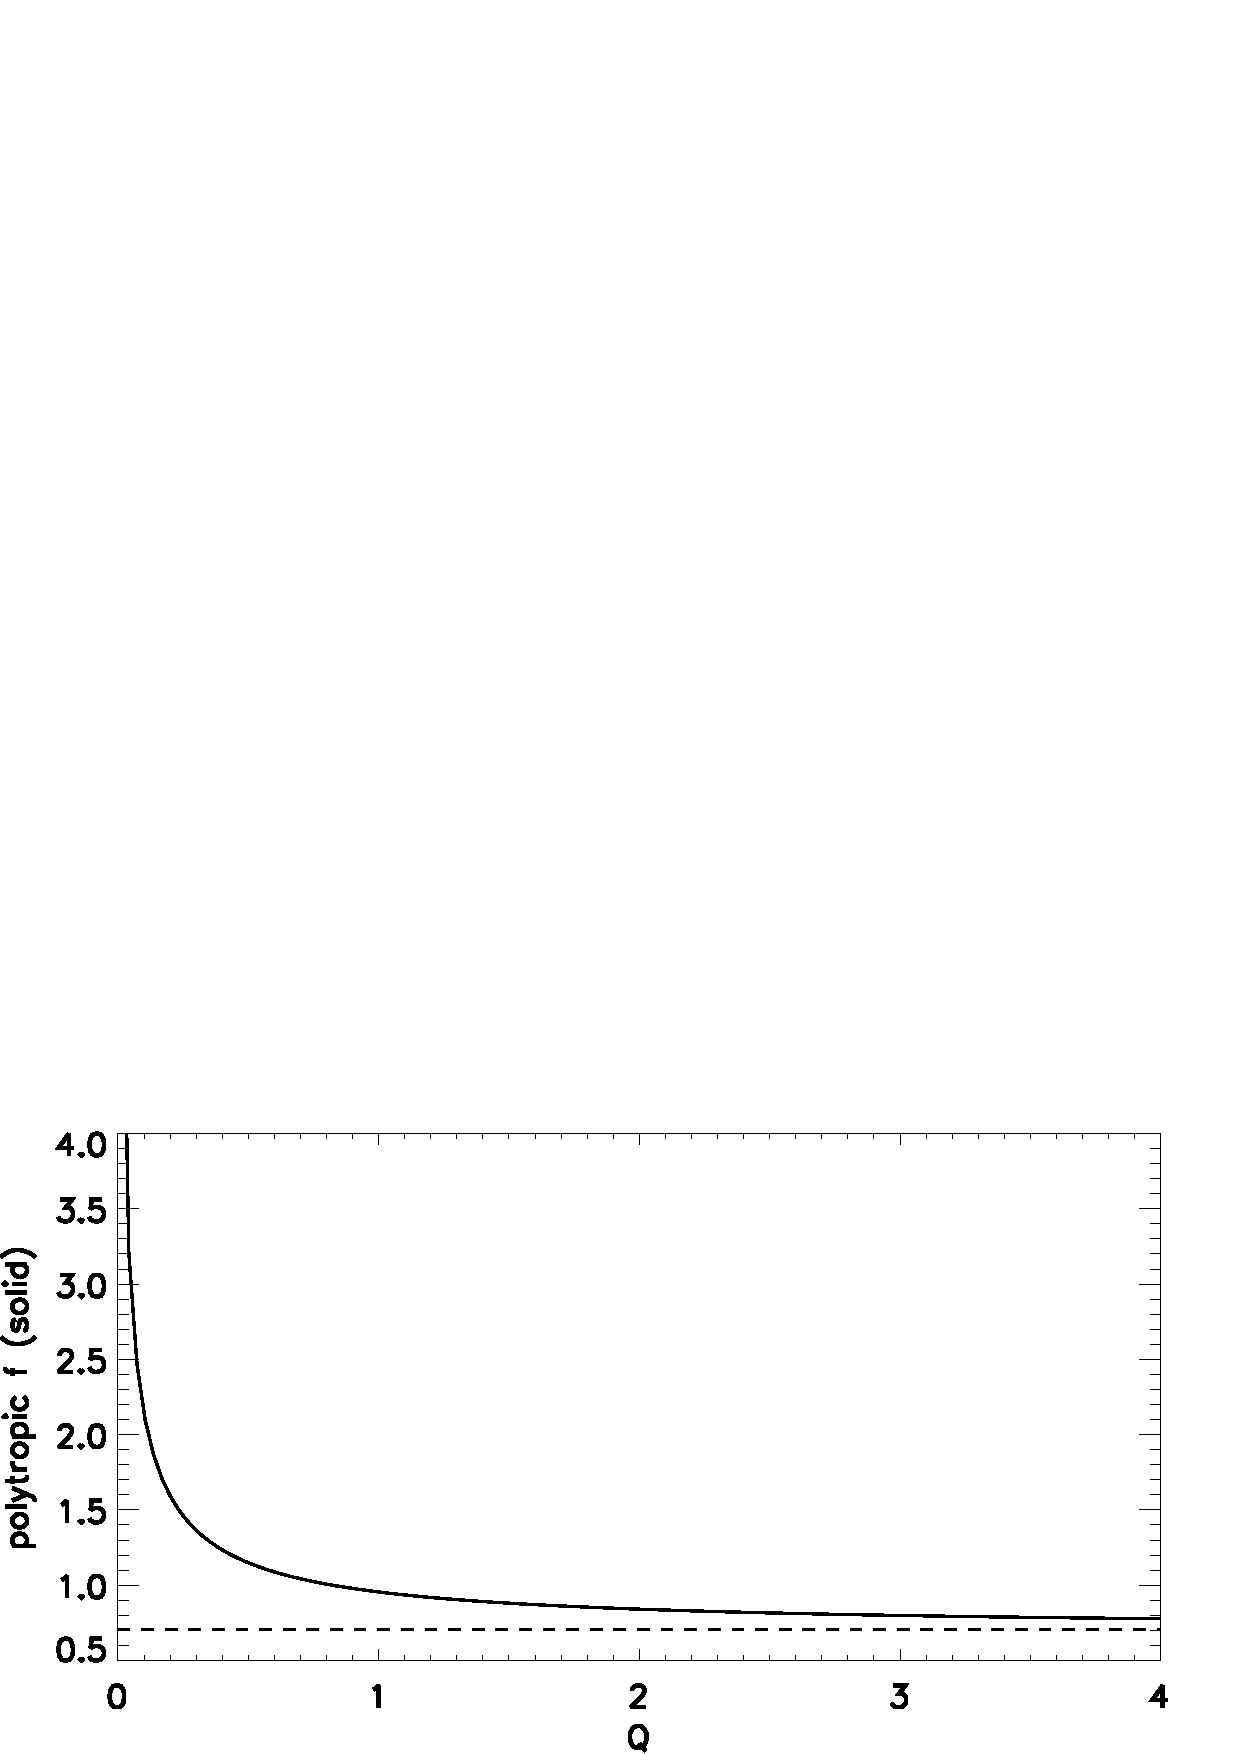
\includegraphics[width=\linewidth]{figures/plot_fq}
  \caption{The function $f(Q)$ describing vertical hydrodstatic 
    equilibrium in self-gravitating polytropic disks (solid line). The
    horizontal dashed line is the asymptotic value of $1/\sqrt{2}$ for
    large $Q$.  
    \label{plot_fq}}
\end{figure}

\section{Relation between $Q$ and the Toomre parameter}\label{q3d2d}
The Toomre parameter defined for razor-thin disks is 
\begin{align} 
  Q_\mathrm{2D}\equiv \frac{\kappa c_s}{\pi G\Sigma},  
\end{align}
where $\Sigma$ is the total column density. To relate our
self-gravity parameter $Q$ and $Q_\mathrm{2D}$, we replace $c_s$ by
$\overline{c_s}\equiv\int\rho c_s dz/\int\rho dz$, and 
$\kappa$ by $\Omega$, giving
\begin{align}
  Q_\mathrm{2D} = 2Qf \frac{\int_0^1
    \hat{\rho} \hat{c}_s
    d\hat{z}}{\left(\int_0^1 \hat{\rho} d\hat{z}\right)^2},   
\end{align}
where each term on the right-hand-side is non-dimensionalized (see
\S\ref{non-dim}). Fig. \ref{plot_q3d2d} plots this relation 
for isothermal and polytropic disks.  

\begin{figure}
  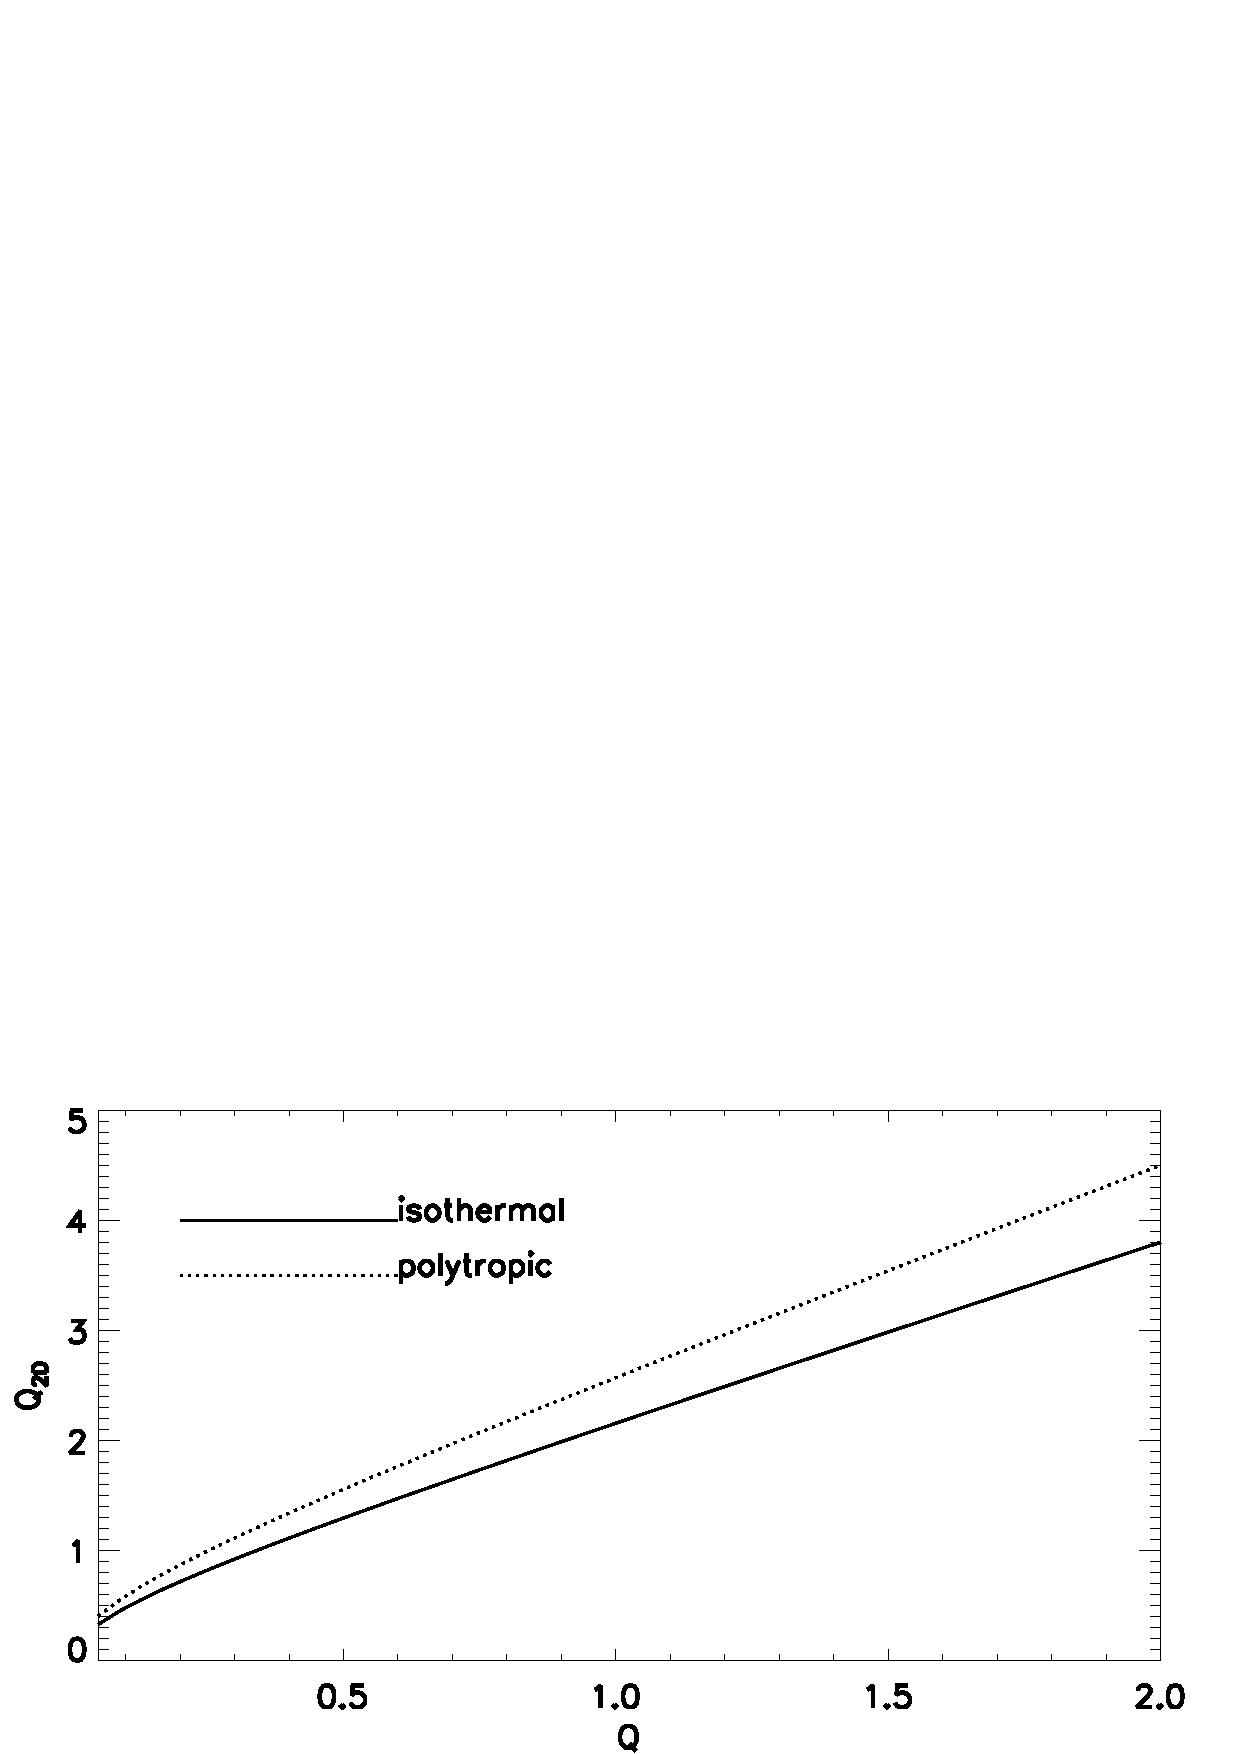
\includegraphics[width=\linewidth]{figures/q2d_iso}
  \caption{Relation between the self-gravity parameter $Q$ used in
    this paper and the Toomre parameter $Q_\mathrm{2D}$ for razor-thin
    disks. 
    \label{plot_q3d2d}}
\end{figure}


\section{Reduction to linear hydrodynamics}\label{reduction} 
Our task here is to remove the magnetic field and vertical velocity
perturbations from the linearized equations. Let us first define operators
\begin{align}
  D_0 = 1, \quad D_1 = \frac{\rho^\prime}{\rho} + \frac{d}{dz}, \quad
  D_2 = \frac{\rho^{\prime\prime}}{\rho} +
  \frac{2\rho^\prime}{\rho}\frac{d}{dz} + \frac{d^2}{d z^2},
\end{align}
and 
\begin{align}
  \overline{D}_0 = \eta D_0, \quad \overline{D}_1 = \eta^\prime D_0 + \eta
  D_1,\quad \overline{D}_2 = \eta^{\prime\prime} D_0 + 2\eta^\prime D_1 +
  \eta D_2. 
\end{align}
And we define the variables
\begin{align}
  &U \equiv \imgi\sigma\dvx - 2\Omega\dvy + \imgi k_x \w,\\
  &V \equiv \imgi\sigma\dvy + \frac{\kappa^2}{2\Omega}\dvx.
\end{align}

We first express the continuity equation in terms of horizontal
velocity, density and potential perturbations. 
The vertical velocity perturbation is 
\begin{align}
  \dvz = \frac{\imgi}{\sigma}\left(\w^\prime + \epsilon V\right),  
\end{align}
where the linearized $y$ momentum equation was used (i.e. eliminating
$\dby^\prime$ between Eq. \ref{lin_vy} and Eq. \ref{lin_vz}). 
Inserting this into the linearized continuity equation
(Eq. \ref{lin_cont}), we obtain
\begin{align}
0 = W^{\prime\prime} + \left(\ln{\rho}\right)^\prime W^\prime +
\frac{\sigma^2}{c_s^2}W +  \dphi^{\prime\prime} + \left(\ln{\rho}\right)^\prime \dphi^\prime
 + \sigma k_x \dvx + \epsilon D_1 V.
%  0=  W^{\prime\prime} + \left(\ln{\rho}\right)^\prime W^\prime +
%  \frac{1}{c_s^2f^2}\left(\frac{\rho}{Q} + \sigma^2\right)W +
% \left(\ln{\rho}\right)^\prime\dphi^\prime + k_x^2\dphi + \frac{\sigma
%    k_x}{f}\dvx.\label{final_w}
\end{align}

Next, we examine separately the cases of a vertical field with
variable resistivity and that of a tilted field with uniform
resistivity. (A similar procedure can be performed in
the general case of a tilted field with variable resistivity.) 

\subsection{Vertical field with variable resistivity}
First consider $\epsilon = 0$ and $\eta=\eta(z)$ in the linearized
equations. Denoting the $n^\mathrm{th}$ vertical derivative as $^{(n)}$, the
equations of motion give
\begin{align}
  &\dbx^{(n)} = \frac{\mu_0\rho}{B_z}D_{n-1}U + \imgi k_x \dbz^{(n-1)},\label{bx_eq}\\
  &\dby^{(n)} = \frac{\mu_0\rho}{B_z}D_{n-1}V,\label{by_eq}
\end{align}
for $n\geq1$. Differentiating the divergence-free condition for the magnetic
field gives
\begin{align}
  \imgi k_x \dbx^{\prime} + \dbz^{\prime\prime} = 0.   
\end{align}
We insert the expression for $\dbx^\prime$ from Eq. \ref{bx_eq} and the
expression for $\dbz^{\prime\prime}$ from the $z$ component of the
linearized induction equation (Eq. \ref{induct_vert}) to obtain
\begin{align}\label{bz_eq}
  -\sigma\dbz^{(n)} = k_x B_z \dvx^{(n)} + k_x\frac{\mu_0\rho}{B_z}\overline{D}_nU. 
\end{align}

%\subsection{Eliminating $\dbx$}
Inserting the above expressions for $\dbx^{\prime\prime}$,
$\dbx^\prime$ (Eq. \ref{bx_eq}) and $\dbz^\prime$  (Eq. \ref{bz_eq})
into the right-hand-side of the $x$-induction equation (Eq. \ref{induct_x} ) gives   
\begin{align}
  \imgi\sigma \dbx =
  B_z\dvx^\prime + \frac{\mu_0\rho}{B_z}\overline{D}_1U. \label{bx_expression}
\end{align}
($\bar{\sigma}\neq0$ has been assumed to obtain this.) We
differentiate this expression with respect to $z$ and eliminate the
resulting $\dbx^\prime$ using Eq. \ref{bx_eq}, to obtain
\begin{align}
%  0 = B_z\dvx^{\prime\prime} -
%  k_x^2B_z\dvx + \frac{\mu_0\rho}{B_z}\left(\overline{D}_2 - k_x^2 \overline{D}_0
%    - \imgi\sigma D_0\right)U. \label{final_vx} 
  0 = v_A^2\left(\dvx^{\prime\prime} -
  k_x^2\dvx\right) + \left(\overline{D}_2 - k_x^2 \overline{D}_0
    - \imgi\sigma D_0\right)U. \label{final_vx} 
\end{align}

%\subsection{Eliminating $\dby$}
We follow a similar procedure as above to remove $\dby$. 
We use Eq. \ref{bx_expression} and Eq. \ref{by_eq} to 
eliminate $\dbx,\dby^\prime$ and $\dby^{\prime\prime}$ from the
right-hand-side of the $y$-induction equation (Eq. \ref{induct_y}), 
%\begin{align}
%  &\imgi\bar{\sigma}\dby = f\dvy^\prime - \imgi
%  S\frac{\dbz^\prime}{k_x} +
%  \eta\dby^{\prime\prime}+\eta^\prime\dby^\prime.  
%\end{align}
%We can now insert expressions for the magnetic field derivatives using
%Eq. \ref{by_eq} and \ref{bz_eq} to obtain an expression for $\dby$, 
\begin{align}
  \imgi\bar{\sigma}\dby = B_z\dvy^\prime + \frac{\imgi S}{\sigma}\left(
    B_z\dvx^\prime + \frac{\mu_0\rho}{B_z}\overline{D}_1U\right) +
  \frac{\mu_0\rho}{B_z}\overline{D}_1V. \label{by_expression}
\end{align}
We differentiate this expression with respect to $z$, then eliminate 
$\dby$ and  $\dby^\prime$ from the left-hand-side of the resulting
expression using Eq. \ref{by_expression} and 
Eq. \ref{by_eq}, respectively. We obtain
\begin{align}
0 = v_A^2\left(\dvy^{\prime\prime} -
\frac{\sbar^\prime}{\sbar}\dvy^\prime\right)  
+ \frac{\imgi S v_A^2}{\sigma}\left(\dvx^{\prime\prime} -
\frac{\sbar^\prime}{\sbar}\dvx^\prime\right) + \frac{\imgi
  S}{\sigma}\left(\overline{D}_2 -
    \frac{\sbar^\prime}{\sbar}\overline{D}_1 \right)U 
+\left(\overline{D}_2 -
    \frac{\sbar^\prime}{\sbar}\overline{D}_1 - \imgi\sbar D_0 \right)V. \label{final_vy}
%0 = B_z\left(\dvy^{\prime\prime} -
%\frac{\sbar^\prime}{\sbar}\dvy^\prime\right)  
%+ \frac{\imgi S B_z}{\sigma}\left(\dvx^{\prime\prime} -
%\frac{\sbar^\prime}{\sbar}\dvx^\prime\right) + \frac{\imgi
%  S}{\sigma}\frac{\mu_0\rho}{B_z} \left(\overline{D}_2 -
%    \frac{\sbar^\prime}{\sbar}\overline{D}_1 \right)U 
%+\frac{\mu_0\rho}{B_z} \left(\overline{D}_2 -
%    \frac{\sbar^\prime}{\sbar}\overline{D}_1 - \imgi\sbar D_0 \right)V. \label{final_vy}
%
%  0 =& \frac{f^2}{\beta\rho}\left(\dvy^{\prime\prime} -
%  \frac{\bar{\sigma}^\prime}{\bar{\sigma}}\dvy^\prime\right) 
%  + \sbar\sigma D_0\dvy  + \frac{\imgi 
%    S}{\sigma}\frac{f^2}{\beta\rho}\left(\dvx^{\prime\prime} -
%    \frac{\sbar^\prime}{\sbar}\dvx^\prime\right) -
%    \frac{\imgi\sbar\kappa^2}{2}D_0\dvx \notag\\
%    & + \left(\overline{D}_2 -
%    \frac{\sbar^\prime}{\sbar}\overline{D}_1\right)\left[\imgi\left(\sigma
%      - \frac{2S}{\sigma}\right)\dvy + \left(\frac{\kappa^2}{2} -
%      S\right)\dvx - \frac{Sfk_x}{\sigma}\w\right]. \label{final_vy}
\end{align}

Eq. \ref{final_vx} and \ref{final_vy} constitutes the first two
linearized equations to be solved.

\subsection{Tilted field with uniform resistivity}
Here we allow $\epsilon\neq 0$ but take $\eta$ to be constant. We
first obtain expressions for $\dbx$ and $\dby$. Differentiating
the $x$ momentum equation and replacing the resuting $\dbz^\prime$
using the divergence-free condition and $\dby^\prime$ using the $y$
momentum equation, we obtain an expression for $\dbx^{\prime\prime}$
which can be inserted into the $x$ induction equation. This gives
\begin{align}
  \imgi\sigma\dbx = B_z\dvx^\prime +
  \frac{\eta\mu_0\rho}{B_z}\left( D_1 U + \imgi\epsilon k_x D_0
  V\right).\label{bx_tilted}  
\end{align}
We can insert this into the $y$ induction equation to obtain
\begin{align}
  \imgi\sbar\dby = -B_y\Delta + B_z\dvy^\prime + \frac{\imgi
    S}{\sigma}\left[ B_z \dvx^\prime+ \frac{\eta\mu_0\rho}{B_z}\left( D_1 U + \imgi\epsilon k_x D_0
  V\right)\right] + \frac{\eta\mu_0\rho}{B_z}D_1V,\label{by_tilted}
\end{align} 
where we have also used the derivative of the $y$ momentum equation to
eliminate  $\dby^{\prime\prime}$. Recall $\Delta \equiv i k_x \dvx +
\dvz^\prime$, so that
\begin{align}
  \Delta = \imgi k_x \dvx + \frac{i}{\sigma}\left(\w^{\prime\prime} +
  \epsilon V^\prime\right) = -\left[\frac{\imgi\sigma W}{c_s^2} +
    \frac{\imgi\left(\ln{\rho}\right)^\prime}{\sigma}\left(\w^\prime +
    \epsilon V\right)\right], 
\end{align}
where the second equality results from the continuity equation. 

Now consider
\begin{align}
  \dbx^\prime - \imgi k_x \dbz = \frac{\mu_0\rho}{B_z}D_0U +
  \imgi\epsilon k_x \dby = \frac{\sigma}{\sbar}\dbx^\prime +
  \frac{\imgi k_x^2B_z}{\sbar}\dvx,
\end{align}
where the first equality corresponds to the $x$ momentum equation and
the second equality results from replacing $\dbz$ using the $z$
induction equation. We can now use the above expressions for $\dbx$
and $\dby$ (Eq. \ref{bx_tilted}--\ref{by_tilted}) to obtain
\begin{align}
0 = &v_A^2\left[k_x^2\left(1+\epsilon^2\right)\dvx - \frac{\epsilon k_x
  S}{\sigma}\dvx^\prime - \dvx^{\prime\prime}\right] + \imgi\epsilon
k_x v_A^2 \dvy^\prime + \frac{\epsilon^2 k_x
  v_A^2}{\sigma}\left(\w^{\prime\prime} + \epsilon V^\prime\right) 
\notag\\ &-\left[\eta\left(D_2 + \frac{\epsilon k_x S}{\sigma}D_1\right) -
  \imgi\sbar D_0 \right]U %\notag\\
- \frac{\imgi\epsilon^2k_x^2S}{\sigma}\eta D_0V.
\end{align}
%We can now use the above expression for $\dbx,\dby$ to eliminate
%$\dbx^\prime$ and $\$ in the $x$ momentum equation  
%\begin{align}
%  \dbx^\prime - \imgi k_x\dbz = \frac{}{}
%\end{align}

Similarly, we differentiate Eq. \ref{by_tilted} and use the $y$
momentum equation to eliminate $\dby^\prime$ to obtain
\begin{align}
0 = &v_A^2\dvy^{\prime\prime} + \frac{\imgi S}{\sigma}v_A^2
\dvx^{\prime\prime} +\frac{\imgi S}{\sigma}\eta D_2U +
\left\{\eta\left(D_2 - \frac{\epsilon k_x S}{\sigma} D_1\right) +
  \imgi\left[\frac{\epsilon^2v_A^2\left(\ln{\rho}\right)^{\prime\prime}}{\sigma}
    - \sbar\right]D_0\right\}V \notag\\ &+ \imgi\epsilon
  v_A^2\left\{\frac{\sigma}{c_s^2}\left[W^\prime -
    \left(\ln{c_s^2}\right)^\prime W\right] +
    \frac{1}{\sigma}\left[\left(\ln{\rho}\right)^\prime(\w^{\prime\prime}
      + \epsilon V^\prime)
      +\left(\ln{\rho}\right)^{\prime\prime}\w^{\prime} \right]\right\}.    
\end{align}

%\subsection{Non-dimensionalization}
%In practice we solve the linearized equations in non-dimensional form,
%by defining
%We further write 
%\begin{align}
%  &z=\hat{z}H,\quad k_x =  \hat{k}_x/H,\quad \sigma = \hat{\sigma}\Omega,
%  \quad \delta\bm{v} = \csmid 
%  \delta\hat{\bm{v}}, \\ 
%  &\delta\bm{B} = B\delta\hat{\bm{B}},\quad
%  \delta\rho = \rho\hat{W}/\hat{c}_s^2,\quad \delta\Phi =
%  \csmid^2\delta\hat{\Phi}, 
%\end{align}
%where we have introduced the non-dimensional enthalpy perturbation
%$\hat{W}$ and the sound-speed $\hat{c}_s=\csmid^{-1}\sqrt{dP/d\rho}$ can be 
%obtained from the equation of state. The background frequencies are
%written $S=\hat{S}\Omega$ and $\Omega_z=\hat{\Omega}_z\Omega$ and the 
%resistivity as $\eta = \hat{\eta}H^2\Omega$. 

%We will now drop the $\hat{\phantom{a}}$ notation. Henceforth it is
%understood that all variables have been appropriately normalized
%(i.e. $\Omega\to 1$ and $H\to 1$), unless otherwise stated.


%tilted field
% calculate b field vertical derivatives carefully
% try no velocity pert at bc
% try anti-aligned field 


\bibliographystyle{apj}
\bibliography{ref}


\end{document}

